% UG project example file, February 2022
%   A minior change in citation, September 2023 [HS]
% Do not change the first two lines of code, except you may delete "logo," if causing problems.
% Understand any problems and seek approval before assuming it's ok to remove ugcheck.
\documentclass[logo,bsc,singlespacing,parskip]{infthesis}
\usepackage{ugcheck}

% Include any packages you need below, but don't include any that change the page
% layout or style of the dissertation. By including the ugcheck package above,
% you should catch most accidental changes of page layout though.
\usepackage{wrapfig}
\usepackage{url}
\usepackage{multirow}
\usepackage{microtype} % recommended, but you can remove if it causes problems
\usepackage{natbib} % recommended for citations
\usepackage{xcolor}
\usepackage{subcaption}
\usepackage{amsmath,amssymb}
\usepackage{tikz}
\usetikzlibrary{arrows.meta,positioning,shapes.geometric,fit,calc}
\usepackage{booktabs} % for \toprule, \midrule, \bottomrule in tables
\usepackage{beamerarticle} % provides beamer environments like columns/column in non-beamer docs
\usepackage{float} % provides the [H] float placement option
\usepackage{graphicx} % for \includegraphics
\usepackage{caption} % for \captionof
\usepackage{kotex} % Korean text support

\begin{document}
\begin{preliminary}

\title{Interpreting RNA Foundation Models: Evidence of Structural Awareness in Pretrained Representations}

\author{Jaehyuk Choi}

% CHOOSE YOUR DEGREE a):
% please leave just one of the following un-commented
\course{Artificial Intelligence}
%\course{Artificial Intelligence and Computer Science}
%\course{Artificial Intelligence and Mathematics}
%\course{Artificial Intelligence and Software Engineering}
%\course{Cognitive Science}
%\course{Computer Science}
%\course{Computer Science and Management Science}
%\course{Computer Science and Mathematics}
%\course{Computer Science and Physics}
%\course{Software Engineering}
%\course{Master of Informatics} % MInf students

% CHOOSE YOUR DEGREE b):
% please leave just one of the following un-commented
%\project{MInf Project (Part 1) Report}  % 4th year MInf students
%\project{MInf Project (Part 2) Report}  % 5th year MInf students
\project{4th Year Project Report}        % all other UG4 students


\date{\today}


\abstract{
RNA foundation models (RNA FMs) pretrained on large sequence corpora are increasingly adopted as representation backbones for RNA secondary structure prediction, often achieving strong results when paired with task-specific prediction heads. As these pipelines become more widespread, a natural question is whether the pretrained representation itself already encodes base-pairing information or whether that information is learned primarily by the prediction head during supervised training. We investigate this by training low-rank bilinear probes on fixed embeddings from five encoder-only models and decoding pairwise base-pairing scores under varying allowed pairing constraints. Recoverability of base-pairing information varies sharply across models. ERNIE-RNA reaches F1 of 0.51 on an in-distribution test set and 0.46 on unseen RNA families, while most other RNA encoders remain below 0.14 under the same protocol. RoBERTa, despite lacking any RNA-specific pretraining, outperforms several RNA-trained encoders, and its advantage grows once allowed pairing constraints compensate for the chemical specificity its representations lack. This shows that measured performance reflects not only what a representation encodes but also how the evaluation is set up.
 
To test whether recovered signals have practical value, we inject probe-derived scores as soft priors into CPLfold. Under CONTRAfold, every encoder benefits, with ERNIE-RNA gaining between 12.8\% and 21.8\% relative F1 over the unaugmented baseline on the out-of-distribution split. Under ViennaRNA, gains are largely confined to ERNIE-RNA and can degrade under distribution shift, suggesting that the usefulness of probe-derived priors depends on the folding backend. Together, these results provide controlled evidence that some, but not all, RNA foundation models encode recoverable and practically useful base-pairing information in their pretrained representations.
}

\maketitle

\newenvironment{ethics}
   {\begin{frontenv}{Research Ethics Approval}{\LARGE}}
   {\end{frontenv}\newpage}

\begin{ethics}
This project was planned in accordance with the Informatics Research
Ethics policy. It did not involve any aspects that required approval
from the Informatics Research Ethics committee.

\standarddeclaration
\end{ethics}


\begin{acknowledgements}
The completion of this dissertation was a journey made possible only through the support and guidance of many remarkable individuals.\\

First and foremost, I would like to express my deepest gratitude to Shay. Your insightful advice and wealth of diverse ideas were the compass that guided this research. Thank you for challenging me to think deeper and for your unwavering mentorship throughout this study.\\

I am also profoundly grateful to Ke, whose expertise and assistance were invaluable. Your support played a crucial role in bringing this work to fruition.\\

To my beloved family, my parents, aunts, and especially my grandmothers, thank you for being my sanctuary. Your unconditional love and silent sacrifices have been the foundation upon which I stand today. \\ 

Finally, to my dear friends, Peter, Hanson, Francesco, Arin, Koe and Jinyoung, thank you for standing by my side and for the joy you brought to my life during this demanding journey.
\end{acknowledgements}


\tableofcontents
\end{preliminary}


\chapter{Introduction}
\label{ch:introduction}

\section{Motivation and context}\label{sec:intro_motivation}

Ribonucleic acid (RNA) molecules serve diverse regulatory and catalytic roles 
that extend well beyond their classical function as intermediaries of genetic 
information \citep{alonso2021mechanisms}. In many cases, RNA function depends on the formation of specific folded structures \citep{tinoco1999how,ganser2019roles}. 
These structures arise from base-pairing interactions between nucleotides (A, U, G, and C). The most common are the canonical Watson–Crick pairs, adenine–uracil (A–U) and guanine–cytosine (G–C), which are typically more thermodynamically stable and therefore more likely to form during RNA folding \citep{sponer2005principles}.
Such structural elements create binding interfaces for interactions with proteins and other RNAs. Beyond this structural role, RNA molecules can adopt multiple conformations, enabling dynamic regulation of these interactions \citep{tants2024rna}. 
The recent success of mRNA-based therapeutics has further underscored the practical relevance of understanding how RNA sequence influences structural stability \citep{chaudhary2021mrna, jin2025mrna}.

Among the different levels of RNA structure, secondary structure, defined by patterns of intramolecular base pairing, provides a particularly useful level of analysis \citep{vandivier2016conservation, bai2016atlas}. It remains simple enough to model directly, while still capturing information relevant to stability and molecular recognition. Accordingly, predicting RNA
secondary structure from sequence has long been a central problem in RNA
bioinformatics \citep{mathews2019benchmark}. The field has been shaped by classical
thermodynamic frameworks such as ViennaRNA \citep{lorenz2011viennarna} as well as
learning-based approaches ranging from early probabilistic models such as CONTRAfold
\citep{do2006contrafold} to more recent deep learning methods including E2Efold,
UFold, and MXfold2 \citep{chen2020e2efold,fu2022ufold,sato2021mxfold2}.

In parallel, the rapid development of large language models (LLMs) has encouraged
the adaptation of language-modelling ideas to biological sequences
\citep{sarumi2024llmbioinformatics}. In this line of work, DNA, RNA, and protein
sequences are treated as discrete sequences over finite alphabets. As a result, models can be pretrained on large unlabelled corpora to learn contextual representations that are reusable across downstream tasks. Early examples include DNABERT for genomic DNA \citep{ji2021dnabert} and Protein Language Models (PLMs) trained
on hundreds of millions of sequences \citep{elnaggar2022prottrans,rives2021biological}.
In the protein domain, representation-level analyses have provided 
evidence that self-supervised pretraining on sequences alone can give rise to embeddings that encode structural properties \citep{rao2021unsupervised, vig2021bertology, lin2023evolutionary}. These results raise the question of whether encoder models pretrained on RNA sequences similarly encode structural properties in their representations.

Within this trend, RNA foundation models \textbf{(RNA FMs)} have emerged as a rapidly developing area, with encoder-based architectures pretrained on large RNA corpora and applied to a range of downstream tasks through nucleotide-level representations \citep{chen2022rnafm,yin2025ernie,penic2025rinalmo}. These tasks include RNA secondary-structure prediction \citep{wang2025depfold, zablocki2025benchmark, singh2019rna} and RNA–protein interaction prediction \citep{tahmid2025birna}. 
% This raises a central question for RNA FMs. 
However, whether RNA FM representations themselves encode base-pairing information without task-specific supervision has not been directly tested. It remains unclear whether pretrained representations already capture which nucleotides pair with each other, or whether such information is learned primarily by the prediction head during supervised training.
This distinction matters because strong downstream performance alone does not demonstrate that
secondary-structure information is already present in the pretrained representations.
Observed gains may instead reflect the capacity of the prediction head or reliance on
features that correlate with structure without directly representing base-pairing patterns
\citep{hewitt2019designing}. Answering this question therefore requires a controlled
representation-level analysis that is separate from end-to-end downstream performance.

This study uses \textbf{structural probing} as a controlled method to study this question \citep{hewitt2019structural}. Since RNA secondary structure is fundamentally defined by base-pairing interactions, we ask \textbf{whether base-pairing information is already encoded in the outputs of pretrained RNA foundation models}. To test this, simple probes are trained to predict pairwise base-pairing scores from model outputs, allowing us to examine whether such information can be recovered and how this varies across layers \citep{hewitt2019structural,belinkov2022probing}. We then ask a second, more practical question, asking \textbf{whether the same probe-derived scores improve RNA structure prediction when incorporated as additional pairwise evidence within a structured folding framework}. This two-stage design separates the
question of what pretrained representations encode from the question of
whether the encoded information is useful in practice.

\section{Goal and research questions}\label{sec:intro_goal_rq}
Building on the motivation and methodological rationale outlined in Section~\ref{sec:intro_motivation}, this study examines whether representations produced by pretrained RNA foundation models encode RNA secondary-structure information, specifically base-pairing patterns. It further investigates whether such information can be leveraged to improve thermodynamic structure prediction.
To address this goal, we consider three research questions. A two-stage experimental approach for investigating them is outlined in Section~\ref{sec:intro_overview}.

\textbf{RQ1: Decodability of base-pairing information.}
Do pretrained RNA FM embeddings encode base-pairing information
that a simple probe can recover without fine-tuning the encoder?
Specifically, we ask whether a low-capacity probe, designed to
minimise the risk of learning structural patterns on its own,
can extract pairwise base-pairing scores from fixed pretrained
representations. We refer to this property as
\textbf{decodability} throughout the thesis, and measure it via \textbf{contact recovery}, the pair-level F1 between probe-predicted and reference base pairs. Within this question, we ask: 
% (Sections~\ref{sec:results_probe_unconstrained}--\ref{sec:results_layer_k}):
\begin{itemize}
  \item[\textbf{(a)}] At which transformer layers is the
    recoverable signal strongest? (Section~\ref{sec:results_layer})
  % \item[\textbf{(b)}] What is the minimum projection rank
  %   required for the probe to recover base-pairing information,
  %   and does increasing rank beyond a small value yield
  %   diminishing returns? (Section~\ref{sec:results_rank})
  \item [\textbf{(b)}] How much probe capacity, projection rank, is needed to recover base-pairing information (Section~\ref{sec:results_rank})?
  \item[\textbf{(c)}] Does imposing chemically plausible
    constraints on the set of permitted base pairs affect decodability, and does this effect differ across models? (Sections~\ref{sec:results_probe_unconstrained},~\ref{sec:results_constraints_best})
\end{itemize}

\textbf{RQ2: Out-of-distribution (OOD) robustness.}
Do the decoded base-pairing signals persist when evaluated on RNA
families unseen during probe training, or do they degrade substantially
under family-level distribution shift?

\textbf{RQ3: Utility as a folding prior.} 
When probe-derived pairwise scores are injected as soft priors into a structured folding algorithm via an $\alpha$-weighted objective, does the augmented folding algorithm yield measurable improvements over the unaugmented baseline? Are these improvements consistent across folding backends and across both in-distribution and OOD evaluation, which would indicate that the probe signal is robust rather than artefactually aligned with a particular scoring framework? (Section~\ref{sec:results_cplfold_utility})

\section{Approach overview}
\label{sec:intro_overview}
Our analysis proceeds in two stages.
In the first stage, we extract token-level embeddings from each RNA foundation model layer, keeping encoder weights fixed. We then train a low-rank bilinear probe \citep{hewitt2019structural} to produce a pairwise score matrix over nucleotide pairs, interpreted as a contact map of base-pairing preferences. Because RNA contact maps are extremely sparse, with positive pairs constitute roughly 0.2\% of all candidate pairs, we employ balanced pair sampling during training. Evaluation is performed under three allowed \textbf{pairing constraints}, that is, restrictions on which nucleotide pair types are permitted during decoding: 
\textbf{unconstrained} (all pair types permitted),
\textbf{canonical} (Watson--Crick pairs only, A--U and G--C),
and \textbf{canonical+wobble} (Watson--Crick pairs plus G--U
wobble pairs). G--U wobble pairs are non-canonical but are included in the canonical+wobble setting because they occur frequently in natural RNA structures \citep{varani2000gu}.
Predicted structures are obtained via greedy max-one decoding with a threshold selected exclusively on the validation split. All settings (layer, probe rank $k$, pairing constraint, threshold $\tau$) are selected on the validation set and fixed before held-out evaluation on both an in-distribution test set (TS0) and a family-shifted out-of-distribution set (NEW).

In the second stage, we inject probe-derived pairwise scores as soft bonuses into CPLfold \citep{wang2026cplfold}, a structured folding framework that augments its scoring objective with an $\alpha$-weighted prior term. We evaluate two \textbf{folding backends}, the structured folding algorithms into which probe scores are injected: ViennaRNA \citep{lorenz2011viennarna}, which uses thermodynamic energy parameters, and CONTRAfold \citep{do2006contrafold}, which uses a learned scoring function. The prior weight $\alpha$ is swept on the validation split and fixed for all held-out evaluation. The probe supplies local pairwise scores estimating how likely each nucleotide pair is to form a base pair, while the folding backend enforces global structural constraints, such as allowing each nucleotide to participate in at most one pair, to produce a valid secondary structure (Section~\ref{sec:methods_problem}).
% The probe provides local pairwise scores derived from pretrained representations, estimating how likely each nucleotide pair is to form a base pair. The folding backend then enforces global structural constraints, for example, requiring each nucleotide to participate in at most one base pair, to produce a valid secondary structure (Section~\ref{sec:methods_problem}).

% Together, the two stages allow us to assess not only whether structural information is present in pretrained embeddings, but also whether it provides practical value when combined with physics-based or learned folding constraints. Detailed experimental procedures are described in Chapters~\ref{ch:methods} and~\ref{ch:experiments}.
Together, the two stages allow us to assess not only whether structural information is present in pretrained embeddings, but also whether it provides practical value when combined with physics-based or learned folding constraints. A schematic overview of the full pipeline is provided in Figure~\ref{fig:diagram} with details in Chapters~\ref{ch:methods} and~\ref{ch:experiments}.

\section{Contributions}
\label{sec:intro_contrib}
Our main contributions are as follows:
\begin{itemize}

\item We design a probing framework that separates what
pretrained RNA encoders already encode from what task-specific
prediction heads learn during fine-tuning. This framework can
serve as a reusable evaluation tool for comparing the
structural content of RNA encoder representations across models
of different scale and architectural design
(Chapters~\ref{ch:methods} and~\ref{ch:experiments}).

\item Through a controlled comparison of four RNA foundation models and a general-purpose language model (RoBERTa), we provide evidence that base-pairing recoverability varies widely across encoders. ERNIE-RNA encodes substantially more base-pairing information than the other models tested, as measured by probe-recovered F1 without any fine-tuning of the encoder. This suggests that architectural design and pretraining strategy influence how accessible structural information is within pretrained representations
(Sections~\ref{sec:results_probe_unconstrained}--\ref{sec:results_constraints_best}).

\item We find that RoBERTa, a general-purpose language model with no RNA-specific pretraining, outperforms several RNA-trained encoders under our probing setup. Its performance improves further when decoding is restricted to chemically plausible base-pair types, indicating that measured decodability is sensitive to the choice of pairing constraints.
(Sections~\ref{sec:results_constraints_best}
and~\ref{sec:disc_roberta}).

\item We demonstrate that pairwise base-pairing scores extracted by the probe can improve structured RNA folding when added to an existing folding algorithm as soft priors. This shows that structural information present in pretrained representations can be used in practice without retraining either the encoder or the folding backend
(Section~\ref{sec:results_cplfold_utility}).

\end{itemize}

\section{Thesis structure}\label{sec:intro_structure}
\begin{itemize}
    \item \textbf{Chapter~\ref{ch:background} (Background)} reviews RNA secondary structure, foundation models, and probing-based interpretability methods.
    \item \textbf{Chapter~\ref{ch:methods} (Methods)} and \textbf{Chapter~\ref{ch:experiments} (Experiments)} describe the probe design, decoding strategies, and hybrid folding integration, together with dataset construction and the experimental protocol.
    \item \textbf{Chapter~\ref{ch:results} (Results)} presents the main empirical results, including layer-wise and low-rank analyses, OOD evaluation, and downstream folding experiments.
    \item \textbf{Chapter~\ref{ch:discussion} (Discussion)} discusses implications, limitations, and future directions.
\end{itemize}

% ============================================================
% Chapter 2: Background
% ============================================================
\chapter{Background}
\label{ch:background}
This chapter provides the background and related work needed to follow the remainder of the dissertation. We begin with the structural biology of RNA base pairing, then review current approaches to RNA secondary structure prediction, including those that use RNA foundation models. We then introduce probing methods for analysing what pretrained representations encode. The chapter concludes by identifying the gaps that motivate our study.
% ------------------------------------------------------------
\section{RNA secondary structure}
% Ver2.
Ribonucleic acid (RNA) is a single-stranded nucleic acid composed of four nucleotides, Adenine (A), Cytosine (C), Guanine (G), and Uracil (U), and it plays a central role in biological information processing \citep{alonso2021mechanisms}. Beyond its role in storing and transmitting genetic information, RNA can also carry out molecular functions directly through its structure. 
These functions depend on specific folding patterns formed by intramolecular base-pairing interactions, which constitute RNA secondary structure \citep{tinoco1999how, ganser2019roles}.
\label{sec:bg_rna_fundamentals}
\begin{wrapfigure}{r}{0.4\textwidth}
    \centering
    \includegraphics[width=0.3\textwidth]{img/rna_structure.png}
    \caption{An example of RNA secondary structure showing base-pairing interactions (adapted from \citep{sato2021mxfold2}).}
    \label{fig:rna_secondary_structure}
\end{wrapfigure}

% Ver2. 
\textbf{Levels of RNA structure.} RNA Structure is conventionally described at three levels \citep{tinoco1999how,turner2009nndb}: \textbf{Primary}, \textbf{Secondary},
and \textbf{Tertiary} structure. The primary structure is the linear nucleotide sequence
$x = (x_1, \dots, x_n)$, where each $x_i \in \Sigma = \{A,C,G,U\}$. 
Tertiary structure refers to the full three-dimensional geometry of the molecule,
but is experimentally difficult to obtain and computationally expensive to model.

Between these two levels lies RNA secondary structure, which captures the
major base-pairing interactions. A secondary structure can be
represented as a set of base pairs $\mathcal{P} \subseteq \{(i,j) \mid 1 \le i < j \le n\}$, where $(i,j)\in\mathcal{P}$ indicates that nucleotides $i$ and $j$ form a
base pair.

\textbf{Base-pairing types.}
The most common base pairs are the canonical Watson--Crick pairs, which are thermodynamically more stable and account for the majority of naturally observed pairings \citep{sponer2005principles}. Another frequently observed pairing is the G--U wobble pair, which is weaker than canonical pairs but occurs widely in tRNA, rRNA, and other structured RNAs \citep{varani2000gu}. Non-canonical pairings beyond G--U also occur, particularly in tertiary interactions, but are not the focus of this thesis.
 
\textbf{Structural constraints.}
Not every possible pair set corresponds to a physically realisable structure. Constraints on the predicted pair set can be divided into \textbf{local} and \textbf{global} categories. Local constraints restrict which nucleotide pair types are admissible including canonical pairs. Global constraints determine whether a full set of predicted pairs forms a valid structure. One such constraint is the max-one pairing condition, which requires each nucleotide to participate in at most one base pair \citep{zuker1981optimal}. 
Some classical algorithms additionally assume pseudoknot-freeness, prohibiting crossing pairs of the form $(i,j)$ and $(k,\ell)$ with $i<k<j<\ell$, because
allowing pseudoknots makes exact inference NP-hard in the general case
\citep{LyngsoPedersen2000}. However, pseudoknots do occur in biological
RNA structures, and some recent methods, including CPLfold
\citep{wang2026cplfold}, relax this assumption.
Section~\ref{sec:methods_problem} provides further details on how these constraints are handled.

\textbf{Representations.}
Secondary structure is often represented in dot-bracket notation, 
as an arc diagram, or as a contact map $M\in\{0,1\}^{n\times n}$ 
where $M_{ij}=1$ if and only if $(i,j)\in P$ 
\citep{mathews2019benchmark}. In dot-bracket notation, paired 
positions are marked by matching parentheses and unpaired positions 
by dots: for instance, \texttt{((...))} denotes a sequence of 
length seven in which positions 1--2 pair with positions 6--7 and 
positions 3--5 are unpaired.
% ------------------------------------------------------------
\section{RNA secondary structure prediction}
\label{sec:bg_prediction_paradigms}
RNA secondary structure prediction seeks to infer the base-pair set
$\mathcal{P}$ for a given RNA sequence $x$. 
RNA secondary structure captures the major intramolecular base-pairing interactions in a simpler and more computationally accessible form than full three-dimensional tertiary structure. Therefore, it has been the main focus of computational RNA structure prediction for more than four decades \citep{zuker1981optimal,tinoco1999how}.
Experimental methods for determining RNA structure remain difficult to apply at large scale, so computational prediction is still the main practical approach to study RNA structure at scale \citep{mathews2019benchmark}.

Predicted secondary structures inform a range of downstream tasks, from
modelling RNA--protein interactions and identifying regulatory elements
to guiding mRNA sequence design where folding stability directly affects translational efficiency
\citep{chaudhary2021mrna,jin2025mrna}. This broad range of applications has led to continued methodological development, which we review below: (i)~classical thermodynamic energy minimisation,
(ii)~supervised learning from annotated structures, and (iii)~recent
pipelines that use pretrained RNA encoders to generate representations for downstream prediction.

\subsection{Classical thermodynamic models}
\label{sec:bg_thermo}
Classical approaches are based on the principle that RNA tends to fold into thermodynamically stable structures \citep{tinoco1999how}, and accordingly formulate secondary structure prediction as a free-energy minimisation problem \citep{zuker1981optimal}. Under the nearest-neighbor thermodynamic model \cite{turner2009nndb}, each candidate base-pairing structure is assigned a free energy, and the predicted structure is the one with minimum free energy (MFE) \cite{zuker1981optimal}. 
As pseudoknot-free structures can be decomposed recursively, the MFE solution can be found in  polynomial time by dynamic programming, as implemented in ViennaRNA \citep{lorenz2011viennarna}.

Grounded in physical principles, these methods enforce structural constraints and do not require annotated training data, reducing the risk of overfitting compared to supervised approaches \citep{mathews2019benchmark}. Their accuracy, however, depends on the quality of the underlying thermodynamic parameters and on modelling assumptions. A further limitation is that standard dynamic programming formulations assume pseudoknot-free structures, since allowing arbitrary pseudoknots makes exact inference NP-hard \citep{LyngsoPedersen2000}. To address some of these constraints, recent structured decoding frameworks incorporate external pairwise evidence into the folding objective. One such framework is CPLfold, which augments thermodynamic or learned scoring with soft priors derived from experimental or computational sources and additionally supports pseudoknot prediction for long RNAs \citep{wang2026cplfold}. Its use in this study is described in the following chapters.

\subsection{Learning-based approaches}
\label{sec:bg_supervised}
Learning-based approaches treat secondary structure prediction as a structured prediction problem trained on
annotated sequences. CONTRAfold was an early example that replaced manually defined thermodynamic energy models with a discriminative scoring function learned from data, while retaining structured inference \citep{do2006contrafold}.
More recent neural predictors such as UFold \citep{fu2022ufold} estimates pairwise base-pairing probabilities using a U-Net and applies post-processing to enforce constraints. Hybrid approaches that combine learning-based models with thermodynamic modeling have also been proposed. For example, MXfold2 integrates these paradigms to improve robustness while preserving constraint-based decoding \citep{sato2021mxfold2}.

Since these methods are trained on annotated structures, their performance can degrade on RNA families that are not represented in the training set. Several studies of deep learning models for RNA secondary structure prediction have shown that strong within-family accuracy does not translate into reliable cross-family generalisation, which is often the more practically relevant setting \citep{szikszai2022, szikszai2026gauging}.

\subsection{Foundation model-based approaches}
\label{sec:bg_fm_backed}
More recent work combines pretrained RNA sequence encoders with task-specific prediction heads or structured decoders \citep{tahmid2025birna, wang2024rnaernie}. In this approach, the encoder produces contextual nucleotide embeddings from the input sequence, and a downstream predictor, typically trained with supervision, maps these embeddings to base-pairing predictions. DEPfold, for instance, reframes RNA secondary structure prediction as dependency parsing with global constraints while using pretrained encoders as feature backbones \citep{wang2025depfold}. 

However, these approaches face two related difficulties. First, 
generalisation remains challenging. Recent benchmarking of several 
RNA foundation models has shown that performance degrades under 
low-homology conditions \citep{zablocki2025benchmark}. Second, 
even when downstream accuracy is high, it does not by itself 
establish what the pretrained representations contain 
\citep{hewitt2019designing, belinkov2022probing}. Performance gains may reflect structural knowledge learned by the prediction head during supervised training, or the ability of constraint-based decoders to enforce valid structures even when structural signals in the embeddings are weak. Predictive accuracy can therefore become partially decoupled from the structural content of the pretrained representations. This ambiguity motivates the representation-level analysis in this thesis, which separates the question of whether a model predicts correctly from the question of what its pretrained representations actually encode.

\section{RNA FMs and representation learning}
\label{sec:bg_rna_fms}
\subsection{Foundation models for sequence representation learning}
Foundation models for biological sequences are based on the pretraining framework first established in natural language processing (NLP). A model is trained on unlabelled sequence data using a self-supervised objective and then reused for 
downstream tasks, either by fine-tuning or by extracting fixed 
representations \citep{devlin2019bert}. These models are typically 
built on the transformer architecture \citep{vaswani2017attention} and can take several architectural forms, including encoder-only, decoder-only, and encoder-decoder transformers. Encoder-only models produce contextual embeddings at each position and are therefore widely used in embedding-based downstream tasks, while decoder-only and encoder-decoder models
are more commonly used for generation and sequence transformation \citep{devlin2019bert,radford2019gpt2,raffel2020t5}.

BERT-style masked language models are a widely used encoder-only architecture in NLP \citep{devlin2019bert}. They are trained to reconstruct randomly masked tokens from bidirectional context, and in doing so learn per-token representations that can be reused without further training of the encoder. RoBERTa \citep{liu2019roberta} refines BERT by removing the next-sentence prediction objective and training with larger batches and more data. We include RoBERTa in our study as a non-RNA baseline. By evaluating RoBERTa and RNA-specific encoders under the same setup, we test whether RNA pretraining provides a measurable advantage over a general-purpose encoder trained without RNA data.

\subsection{RNA FMs}
RNA FMs adapt this pretraining strategy to RNA sequences, producing contextual nucleotide embeddings that can be reused across downstream tasks \citep{chen2022rnafm, yin2025ernie, penic2025rinalmo}. Existing RNA sequence models span encoder-only, decoder-only, and encoder-decoder architectures.
In this study, we focus on encoder-only models because they 
produce per-token embeddings from bidirectional context, which 
makes them directly amenable to pairwise probing. This is 
relevant for RNA secondary structure, where base-pairing 
interactions can occur between nucleotides that are distant in 
sequence \citep{tinoco1999how}.
We therefore examine four representative encoder-only RNA FMs (Figur~\ref{fig:rna-lm-timeline}), which differ in scale, architectural bias, and pretraining design.

\textbf{RNABERT} \citep{akiyama2022rnabert} is an early BERT-style RNA-specific encoder trained on RNA sequences. It uses six transformer layers and produces 120-dimensional token
embeddings, making it smaller than later RNA FMs. Despite
its smaller scale, it is historically notable as one of the first encoder-only models pretrained specifically on RNA.

\textbf{RNA-FM} \citep{chen2022rnafm} is a larger encoder pretrained on approximately 23~million non-coding RNA sequences, producing 640-dimensional embeddings across 12 transformer layers.
 
\textbf{ERNIE-RNA} \citep{yin2025ernie} retains a 12-layer encoder architecture of similar scale to RNA-FM, while introducing mechanisms motivated by RNA structure. In particular, it uses a pairwise attention bias that promotes attention between positions likely to form base pairs, thereby exposing the encoder to structural proximity signals during pretraining.

\textbf{RiNALMo} \citep{penic2025rinalmo} scales substantially beyond these earlier models to 33~layers and approximately 650~million parameters. It provides a contrast to smaller and more structurally biased encoders when examining how model scale relates to recoverable structural signal.

Other notable encoder-only RNA FMs not evaluated in this study include
Uni-RNA \citep{wang2023unirna}, RNAErnie \citep{wang2024rnaernie}, and
AIDO.RNA \citep{he2025aidorna}, the latter scaling to 1.6 billion
parameters.

\begin{figure}[H]
\centering
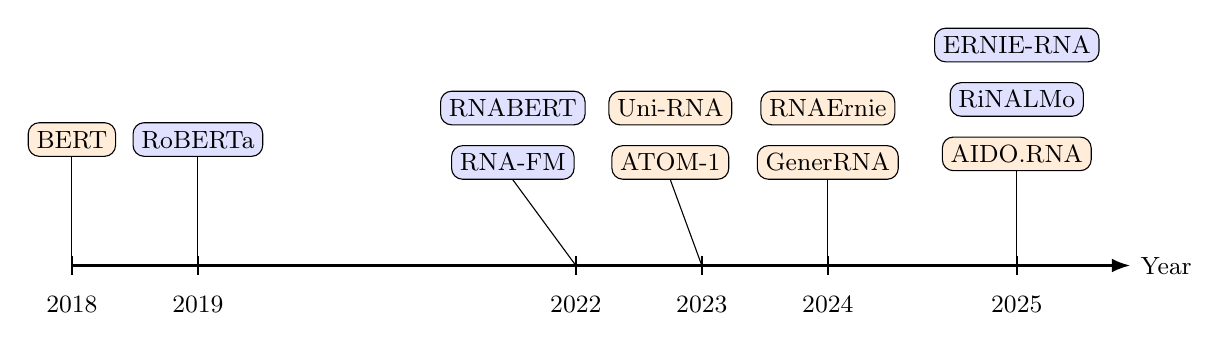
\begin{tikzpicture}[x=1.6cm,y=1.0cm,>=Latex,font=\small]
    \tikzset{
        inTable/.style={draw,rounded corners,fill=blue!12,inner sep=3pt},
        notInTable/.style={draw,rounded corners,fill=orange!15,inner sep=3pt}
    }
    % Timeline axis
    \draw[->,thick] (0,0) -- (8.4,0) node[right]{Year};
    \foreach \x/\yr in {0/2018,1/2019,4/2022,5/2023,6/2024,7.5/2025} {
        \draw[thick] (\x,0.12) -- (\x,-0.12) node[below=4pt]{\yr};
    }
    % 2018
    \node[notInTable] (bert) at (0,1.6) {BERT};
    \draw[thin] (0,0) -- (bert.south);
    % 2019
    \node[inTable] (roberta) at (1,1.6) {RoBERTa};
    \draw[thin] (1,0) -- (roberta.south);
    % 2022
    \node[inTable] (rnabert) at (3.5,2.0) {RNABERT};
    \node[inTable,below=0.25cm of rnabert] (rnafm) {RNA-FM};
    \draw[thin] (4,0) -- (rnafm.south);
    % 2023
    \node[notInTable] (unirna) at (4.75,2.0) {Uni-RNA};
    \node[notInTable,below=0.25cm of unirna] (atomone) {ATOM-1};
    \draw[thin] (5,0) -- (atomone.south);
    % 2024
    \node[notInTable] (rnaernie) at (6,2.0) {RNAErnie};
    \node[notInTable,below=0.25cm of rnaernie] (generrna) {GenerRNA};
    \draw[thin] (6,0) -- (generrna.south);
    % 2025
    \node[inTable] (ernierna) at (7.5,2.8) {ERNIE-RNA};
    \node[inTable,below=0.25cm of ernierna] (rinalmo) {RiNALMo};
    \node[notInTable,below=0.25cm of rinalmo] (aidorna) {AIDO.RNA};
    \draw[thin] (7.5,0) -- (aidorna.south);
\end{tikzpicture}
\caption{Chronological timeline of RNA and general-purpose language
models referenced in this thesis, arranged by publication year. Models
evaluated in this study (Table~\ref{tab:bg_model_summary}) are
highlighted in blue; additional models are in orange.}
\label{fig:rna-lm-timeline}
\end{figure}
% \vspace{-1.5em}

\textbf{Decoder-only.} Decoder-only RNA language models such as GenerRNA \citep{zhao2024generrna} are typically trained
autoregressively and are often used for sequence generation or likelihood
estimation. Because their representations condition only on left context, they are less suited to probing long-range bidirectional dependencies such as those involved in RNA base pairing. We therefore do not evaluate decoder-only models in this study.

\begin{table}[t]
\centering
\small
\caption{Summary of representative BERT-based RNA foundation models.}
\label{tab:bg_model_summary}
\begin{tabular}{lcccc}
\toprule
\textbf{Model} & \textbf{Hidden dim} & \textbf{Layers} & \textbf{Pretraining data (approx.)} & \textbf{Params (approx.)} \\
\midrule
RNABERT & 120 & 6 & $\sim$76k ncRNA seqs & $\sim$0.5M \\
RNA-FM & 640 & 12 & $\sim$23M ncRNA seqs & $\sim$100M \\
ERNIE-RNA & 768 & 12 & large-scale RNA corpus (tens of M) & $\sim$86M \\
RiNALMo & 1280 & 33 & $\sim$36M RNA seqs & $\sim$650M \\
\bottomrule
\end{tabular}
\end{table}
\vspace{-1.0em}
% ------------------------------------------------------------

\section{Interpretability and probing for biological FMs}
\label{sec:bg_interpretability}
The preceding sections reviewed RNA secondary structure and 
modern prediction pipelines, including FM-backed approaches 
(Section~\ref{sec:bg_fm_backed}) that combine pretrained 
encoders with task-specific heads and constraint-based decoding.
As discussed in Section~\ref{sec:intro_motivation}, strong downstream performance alone does not show whether structural information is already encoded in pretrained representations or learned by task-specific heads during supervised training. Addressing this question requires tools that probe representations independently of downstream performance.

\subsection{Representation-level interpretability}
In NLP, interpretability broadly refers to explaining model behavior in a way that helps humans understand why a model produces a particular output for a given input \citep{doshi2017towards,belinkov2022probing}. This goes beyond comparing models' predictive accuracy and instead examines what information is encoded in the representations and how it changes across layers \citep{rogers2020primer,belinkov2022probing}. Interpretability analysis is commonly motivated by reliability and robustness assessment, and evaluation of ethical risks such as bias \citep{ribeiro2016trust,sundararajan2017axiomatic,barocas2016big}. Prior surveys distinguish several levels of analysis, including input-level (which input features matter), representation-level (what information is encoded in hidden states), and mechanism-level (how computations are carried out) \citep{belinkov2019analysis,danilevsky2020survey}. 
This thesis focuses on representation-level interpretability, asking whether pretrained RNA representations encode structural information, which we examine using \textbf{probing}.

\subsection{Probing as a representation-level method}
\label{sec:bg_probing_nlp}
Probing is a widely used method for assessing what information is recoverable from learned representations \citep{conneau2018probing,hewitt2019structural}. 
A simple auxiliary classifier is trained on top of pretrained embeddings that are held fixed to predict a target property. If a simple probe achieves reasonable accuracy, this is taken as evidence that the relevant information is encoded in the representations \citep{hewitt2019designing,belinkov2022probing}.
A central methodological concern in probing is probe capacity. If the probe is too expressive, high accuracy may reflect the probe's own modelling power rather than information present in the representation \citep{hewitt2019designing}. This motivates the use of deliberately simple probes, so that successful recovery can be attributed to the representation itself.

Hewitt and Manning \citep{hewitt2019structural} proposed a structural probe for NLP that learns a low-rank linear transformation of word embeddings under which squared distances correspond to parse tree distances. The probe is parameterised by a single matrix $B \in \mathbb{R}^{k \times D}$, with no nonlinearities, and the rank of $B$ both limits probe complexity and reveals how compactly syntactic structure is encoded in the representation space.

In our setting, the target property is pairwise because RNA base pairing is defined over pairs of nucleotide positions rather than tree distances between words. We therefore adapt the low-rank projection idea into a bilinear scoring function that estimates pairwise base-pairing compatibility. 
By varying the rank parameter k, we can additionally ask how compactly the recoverable signal is distributed in the representation space. Full details of the probe parameterisation are given in Section~\ref{sec:methods_probe}.

\subsection{Interpretability in Biological Foundation Models}
\label{sec:bg_interp_protein}

As biological foundation models are increasingly used as reusable
representation backbones, understanding what their pretrained
representations encode has become an important question
\citep{guo2025foundation,budhkar2025demystifying}. 
This matters most when model-derived signals feed into biological interpretation or serve as priors for downstream analysis.
In such settings, strong predictive performance alone does not establish
what the representations contain, and treating the model as a black box
can limit both interpretability and downstream trustworthiness
\citep{budhkar2025demystifying,zhou2025pathway}.

\textbf{Protein language models.} The most extensive representation-level interpretability work in computational biology has been conducted on protein language models. Attention-based analyses have shown that specific attention heads in
pretrained protein transformers capture structural and functional
properties \citep{rao2021unsupervised,vig2021bertology}. At the representation level, linear classifiers trained on fixed pretrained embeddings have been shown to recover structural properties without any
task-specific fine-tuning \citep{rives2021biological}. 
More recent mechanistic approaches have examined protein representations through feature decomposition, with sparse autoencoders identifying interpretable latent features aligned with structural motifs and functional domains \citep{simon2025interplm}.

\textbf{RNA FMs.}
For RNA, interpretability work has so far focused primarily on
attention-based analyses. Several studies report that individual
attention heads in pretrained RNA encoders correlate with base-pairing
patterns \citep{zhang2024rnamsm,galanos2025rna,yin2025ernie}. 
These findings are informative but address a different question from ours. Attention weights reflect how a model distributes focus during computation, but high attention between two positions does not guarantee that the corresponding token embeddings encode recoverable base-pairing information \citep{jain2019attention}.

Probing offers a more direct test by training a constrained classifier
on fixed embeddings \citep{hewitt2019structural}, but has seen only
limited application to RNA. ATOM-1 recovered base-pairing information using small probe networks on embeddings extracted from its pretrained encoder \citep{celaj2023atom1}. However, the analysis was limited to a single encoder-decoder model, rather than a comparative study across the encoder-only architectures examined in this thesis. A recent benchmark 
compared embeddings from several RNA language models 
for secondary structure prediction, but used a high-capacity 
prediction head that makes it difficult to attribute 
performance to the representations alone 
\citep{zablocki2025benchmark}. To our knowledge, no study has applied capacity-controlled pairwise probing, where the probe's rank is explicitly constrained to limit its own learning capacity, systematically across encoder-only RNA foundation models.

\section{Research gaps and rationale for this study}
\label{sec:bg_gaps}
FM-backed prediction pipelines achieve strong accuracy on RNA secondary structure benchmarks \citep{wang2025depfold,chen2022rnafm,yin2025ernie}. However, as discussed in Section~\ref{sec:bg_fm_backed}, this accuracy reflects the combined contributions of the pretrained encoder, the prediction head, and the decoder. As a result, it remains unclear whether pretrained representations themselves already encode base-pairing information, or whether this information is introduced mainly during supervised training or decoding. Some prior work has addressed this question indirectly. Attention-based analyses \citep{zhang2024rnamsm,galanos2025rna,yin2025ernie} show that certain attention heads correlate with base-pairing patterns. Yet attention weights indicate how a model allocates focus during computation, rather than what is stored in the nucleotide-level representations passed to downstream components \citep{jain2019attention}.

As discussed in Section~\ref{sec:bg_interp_protein}, ATOM-1 applied probing to representations from its own pretrained encoder \citep{celaj2023atom1}, but differs from the setting considered here in several ways. ATOM-1 is an encoder-decoder model whose encoder outputs, for each pair of positions (i,j), a dedicated 256-dimensional feature vector. The probe is then applied to these precomputed pairwise features. In encoder-only models, by contrast, the encoder produces only a single embedding vector per nucleotide, and any pairwise information must be recovered by the probe from these per-token representations. Second, ATOM-1 used a 2.6M-parameter MLP as its probe, which is expressive enough to learn non-trivial patterns on its own, making it harder to attribute performance to the representation rather than the probe. Third, the analysis covered a single model with no cross-encoder comparison, no layer-wise analysis, and no family-level out-of-distribution evaluation.

A further question is whether recovered signals have practical 
value beyond diagnostic interest. Probing measures 
recoverability under a particular classifier, and as Belinkov 
\citep{belinkov2022probing} note in a broader survey of probing 
methodology, high probe accuracy does not by itself establish 
that the recovered information is useful for downstream tasks. 
No prior work has tested whether probe-derived pairwise scores 
can serve as soft priors within a structured folding backend, or 
whether such integration remains effective on RNA families not 
seen during probe training.

These gaps motivate the two-stage design of this thesis. If 
pretrained representations already encode base-pairing 
information, that signal could be reused as a lightweight 
structural prior across prediction pipelines, reducing reliance 
on task-specific fine-tuning. This is increasingly relevant as 
RNA FMs are adopted in applied settings such as mRNA design and 
functional annotation. In the protein domain, structural 
information has been shown to emerge from sequence-only 
pretraining \citep{rives2021biological,lin2023evolutionary}, but 
whether an analogous phenomenon occurs in encoder-only RNA 
language models remains poorly understood. By evaluating both 
recoverability and downstream utility, this thesis aims to 
provide a more complete picture than either analysis alone. The 
concrete experimental approach is presented in the following 
chapters.

\chapter{Methods}
\label{ch:methods}
This chapter describes the methodological framework of the thesis. The analysis proceeds in two stages. The first stage trains a capacity-controlled pairwise probe on representations from pretrained encoders, held fixed, to assess whether base-pairing information is recoverable without task-specific adaptation of the encoder (Sections~\ref{sec:methods_embeddings}--\ref{sec:methods_decoding_probeonly}). The second stage incorporates the probe-derived signal into CPLfold~\citep{wang2026cplfold} as a soft prior, testing whether the recovered information improves thermodynamic structure prediction beyond the unaugmented baseline (Sections~\ref{sec:methods_cplfold}).

Details of the datasets, model configurations, including baselines, and hyperparameter search spaces are provided in Chapter~\ref{ch:experiments}.

\section{Problem formulation and scope}
\label{sec:methods_problem}
Let $x=(x_1,\dots,x_L)$ be an RNA sequence of length $L$, where each nucleotide $x_i \in \{\mathrm{A,C,G,U}\}$. We represent the
reference secondary structure as a set of annotated base pairs, $\mathcal{P}_{\mathrm{true}} \subseteq \{(i,j)\mid 1 \le i < j \le L\}$,
% \begin{equation}
% \mathcal{P}_{\mathrm{true}} \subseteq \{(i,j)\mid 1 \le i < j \le L\},
% \end{equation}
where \((i,j) \in \mathcal{P}_{\mathrm{true}}\) denotes that nucleotides
at positions \(i\) and \(j\) form a base pair in the reference structure.
Our objective is to predict a base-pair set
\(\mathcal{P}_{\mathrm{pred}}\) that satisfies the following
structural constraints.

\textbf{Local constraints.} As introduced in Section~\ref{sec:bg_rna_fundamentals}, local constraints restrict which nucleotide pair types are admissible during decoding among predicted nucleotide pairs. In RNA,
the canonical Watson-Crick pairs (A-U and G-C) are the most thermodynamically stable and account for most observed base pairs, while G-U wobble pairs are non-canonical but still naturally occurring \citep{varani2000gu,turner2009nndb}. \textbf{Unconstrained} allows all nucleotide pair types and \textbf{Canonical-only} restricts candidates to Watson-Crick pairs. \textbf{Canonical+wobble} additionally permits GU and UG. Treating canonical-only and canonical+wobble as separate conditions allows us to isolate the effect of permitting wobble pairs, rather than folding all chemically plausible pairs into a single constrained setting. More broadly, comparing all three settings helps distinguish pair recovery that is supported by the score matrix itself from gains that come from the decoder excluding chemically implausible candidates.

\textbf{Global constraints.} We impose only the max-one pairing
constraint (Section~\ref{sec:bg_rna_fundamentals}), requiring that each
nucleotide participates in at most one predicted base pair. We do not
enforce pseudoknot-freeness. Pseudoknots are naturally occurring recurring structural patterns present in a substantial fraction of known RNA structures. Several recent methods similarly omit this constraint by treating structure prediction as pairwise classification \citep{singh2019rna,fu2022ufold,wang2026cplfold}. More importantly for our
purposes, keeping the decoder minimal ensures that performance
differences across models can be attributed to the representations
rather than to structural inductive bias in the decoding algorithm.

Accordingly, $\mathcal{P}_{\mathrm{pred}}$ is constructed from the set of all nucleotide pairs subject to the local and global constraints defined above, reducing RNA secondary structure prediction to pairwise contact prediction under explicit constraints. Within this formulation, the thesis addresses two questions in separate stages. The first asks whether base-pairing information is recoverable from pretrained representations (Sections~\ref{sec:methods_embeddings}-\ref{sec:methods_decoding_probeonly}). The second asks whether the recovered signal improves prediction when integrated into an existing structured folding backend (Sections~\ref{sec:methods_cplfold}).

\subsection{Overview of the experimental pipeline}
\begin{figure}[H]
    \centering
    \includegraphics[width=\linewidth]{img/diagram.pdf}
    \caption{Overview of the experimental pipeline.}
    \label{fig:diagram}
\end{figure}

Figure~\ref{fig:diagram} shows the overall experimental pipeline. In \textbf{Phase~1}, a frozen encoder $f_{m,\ell}$ converts an input RNA sequence $x$ into per-nucleotide embeddings $\mathbf{H}$, as described in Sections~\ref{sec:methods_embeddings} and~\ref{sec:exp_models}. In \textbf{Phase~2}, a low-rank bilinear probe is trained on these embeddings to produce a dense pairwise score map $\mathbf{P}$ with entries $p_{ij}$, and the best configuration is selected on VL0 following the procedure in Sections~\ref{sec:methods_probe} to~\ref{sec:methods_training} and Sections~\ref{sec:exp_selection} to~\ref{sec:exp_selection_criterion}. In \textbf{Phase~3a}, the score map $\mathbf{P}$ is decoded using \textbf{greedy max-one decoding} (Figure~\ref{fig:maxone_decoding}) with threshold $\tau_{\mathrm{decode}}$ to obtain a predicted base-pair set $\mathcal{P}_{\mathrm{pred}}$, without using a structured folding backend, as described in Sections~\ref{sec:methods_decoding_probeonly} and~\ref{sec:exp_probe_only_eval}. In \textbf{Phase~3b}, thresholded probe scores with $p_{ij} \ge \tau_{\mathrm{export}}$ are exported as weighted bonuses. CPLfold predicts a globally consistent secondary structure by optimizing an augmented objective with trade-off weight $\alpha$ under the ViennaRNA or CONTRAfold backend, as described in Sections~\ref{sec:methods_cplfold} and~\ref{sec:exp_alpha}. All configuration decisions are made on VL0, and TS0 and NEW are evaluated only after these settings have been fixed.

\section{Representation extraction}
\label{sec:methods_embeddings}

For each encoder \(m\) and layer \(\ell\), we extract per-nucleotide
representations by passing an input RNA sequence through the
pretrained model,
\begin{equation}
f_{m,\ell}: x \mapsto \mathbf{H}^{(m,\ell)} \in \mathbb{R}^{L \times D},
\end{equation}
where \(D\) is the hidden dimension and \(L\) is the sequence length
after removing non-nucleotide special tokens. We write the
representation at position \(i\) as \(\mathbf{h}_i\in\mathbb{R}^D\), hence

\begin{equation}
\mathbf{H}^{(m,\ell)} =
\begin{bmatrix}
\mathbf{h}_1^\top\\
\vdots\\
\mathbf{h}_{L}^\top
\end{bmatrix}.
\end{equation}

Throughout this study, encoder weights are held fixed, and only the probe parameters described in Section~\ref{sec:methods_probe} are updated during training. Keeping the encoder fixed is a deliberate design
choice that follows the standard probing paradigm introduced in earlier work~\citep{alain2017understanding} and formalised in subsequent studies~\citep{hewitt2019structural,belinkov2022probing}. Any
base-pairing signal recovered by the probe can therefore be attributed
to information already present in the pretrained representations. Since the encoder receives no gradient updates during probe training, the result cannot be explained by task-specific fine-tuning. Holding the encoder fixed also ensures a fair
comparison across models and layers, as every encoder is evaluated
through an identical downstream evaluation setup.

\section{StructuralContactProbe: a low-rank pairwise probe}
\label{sec:methods_probe}

To test whether base-pairing information is recoverable from these representations, we design a lightweight pairwise probe referred to as the \textbf{StructuralContactProbe}. The probe is intentionally low-capacity, expressive enough to read out pairwise compatibility from the embeddings but not so expressive that it could learn complex structural patterns independently of the encoder. If the probe is too expressive, it may learn the task independently of the representation, making it impossible to determine what the encoder itself contributes~\citep{pimentel2020pareto, hewitt2019designing,belinkov2022probing}.

The design builds on the structural probe of Hewitt and Manning~\citep{hewitt2019structural}, which learns a low-rank linear map to test whether syntactic tree distances are reflected in representation geometry. We retain the low-rank projection but replace distance regression with a symmetric bilinear contact score, described in Section~\ref{sec:methods_probe_scoring}. The target property here is not a continuous distance between tokens but a binary label indicating whether two nucleotide positions form a base pair.

\subsection{Projection and scoring}
\label{sec:methods_probe_scoring}
For each position $i$, let $\mathbf{h}_i \in \mathbb{R}^{D}$ denote
the embedding extracted in Section~\ref{sec:methods_embeddings}. The
probe learns a single matrix $\mathbf{B} \in \mathbb{R}^{D \times k}$ that projects each
embedding into a $k$-dimensional subspace. The projected representation is
\begin{equation}
\mathbf{z}_i = \mathbf{B}^{\top}\mathbf{h}_i \in \mathbb{R}^{k},
\qquad
\mathbf{B} \in \mathbb{R}^{D \times k}.
\end{equation}
For each candidate pair $(i,j)$ with $i<j$, the probe assigns a symmetric compatibility logit
\begin{equation}
s_{ij} = \mathbf{z}_i^\top \mathbf{z}_j
       = \mathbf{h}_i^\top (\mathbf{B}\mathbf{B}^\top)\mathbf{h}_j,
\end{equation}
and converts logits to probabilities via a sigmoid,
\begin{equation}
p_{ij} = \sigma(s_{ij}) = \frac{1}{1+\exp(-s_{ij})}.
\end{equation}
Base pairing is inherently a pairwise property, and the bilinear formulation reflects this by computing each score from exactly two nucleotide representations. The rank parameter $k$ provides an explicit capacity control. By constraining the probe to a low-dimensional latent subspace, we test whether base-pair compatibility is recoverable through a simple low-rank interaction rather than a highly expressive classifier~\citep{hewitt2019designing,pimentel2020pareto}.

\section{Probe training}
\label{sec:methods_training}

\subsection{Pairwise labels}
\label{sec:methods_training_labels}

For each valid candidate pair $(i,j)$, we define a binary label
\begin{equation}
y_{ij} = \mathbb{I}\big[(i,j)\in\mathcal{P}_{\mathrm{true}}\big],
\qquad 1 \le i < j \le L.
\end{equation}
The probe is therefore trained as a binary classifier over nucleotide pairs.

\subsection{Balanced pair sampling}
\label{sec:methods_training_sampling}
As shown in Section~\ref{sec:exp_data_pairspace}, the number of candidate pairs grows quadratically with sequence length, whereas the number of true base pairs remains much smaller. Training over the full pair space would therefore be dominated by non-base-paired pairs. Such class imbalance is common in contact prediction problems and is typically handled through loss weighting or sampling-based rebalancing~\citep{rao2021unsupervised,fu2022ufold}. We address this using balanced pair sampling, where each base-paired pair in a minibatch is matched with one randomly sampled non-base-pair to give a 1:1 ratio of annotated base pairs to sampled non-base-pairs. This prevents the loss from being dominated by non-base-paired pairs and improves optimisation stability in the sparse-label setting. Let $\Omega^+$ and $\Omega^-$ denote the sampled annotated base-pair set and sampled non-base-pair set, respectively, and let $\Omega=\Omega^+\cup\Omega^-$.
Only pairs in $\Omega$ contribute to the training loss. \\

We also experimented with reweighting the positive class in the binary cross-entropy loss as an alternative to sampling-based rebalancing, but observed no improvement, so balanced pair sampling is used throughout.

\subsection{Training objective}
\label{sec:methods_training_loss}
% Let $\Omega(M)$ denote the set of sampled nucleotide pairs drawn from minibatch $M$. The pairwise labels \(y_{ij}\) and the balanced sampling procedure are described in Sections~\ref{sec:methods_training_labels} and~\ref{sec:methods_training_sampling}, respectively. Given the logit scores \(s_{ij}\) defined in Section~\ref{sec:methods_probe_scoring}, we train the probe by minimising binary cross-entropy over \(\Omega(M)\), which is a standard objective for RNA pairwise contact prediction~\citep{fu2022ufold,singh2019rna}. Padding positions and other invalid indices are excluded from both sampling and loss computation.
% \begin{equation}
% \mathcal{L}(M)=
% -\frac{1}{|\Omega(M)|}
% \sum_{(i,j)\in\Omega(M)}
% \left[
% y_{ij}\log \sigma(s_{ij}) + (1-y_{ij})\log\!\big(1-\sigma(s_{ij})\big)
% \right].
% \end{equation}
Let $\Omega(M)$ denote the set of sampled nucleotide pairs drawn from minibatch $M$.
The pairwise labels $y_{ij}$ and the balanced sampling procedure are described in
Sections~\ref{sec:methods_training_labels} and~\ref{sec:methods_training_sampling},
respectively. Given the logit scores $s_{ij}$ defined in
Section~\ref{sec:methods_probe_scoring}, we train the probe by minimising binary
cross-entropy over $\Omega(M)$:
\begin{equation}
\mathcal{L}(M)=
-\frac{1}{|\Omega(M)|}
\sum_{(i,j)\in\Omega(M)}
\left[
y_{ij}\log \sigma(s_{ij}) + (1-y_{ij})\log\!\big(1-\sigma(s_{ij})\big)
\right].
\end{equation}
Binary cross-entropy is a standard objective for pairwise contact
prediction in RNA structure models~\citep{fu2022ufold,singh2019rna}.
Padding positions and other invalid indices are excluded from both
sampling and loss computation.

\section{From probe scores to predicted structures}
\label{sec:methods_decoding}
After training, the probe assigns a probability $p_{ij} = \sigma(s_{ij})$ (Section~\ref{sec:methods_probe_scoring}) to every candidate nucleotide pair $(i,j)$ in a given sequence, producing a pairwise score matrix.
Converting these continuous scores into
discrete base-pair predictions ($\hat{y}_{ij}\in\{0,1\}$), requires decoding. We consider
two settings. In the probe-only setting (Section~\ref{sec:methods_decoding_probeonly}), probe scores are used directly to construct a predicted set of base pairs. This provides a direct measure of what can be recovered from the representations alone. In the hybrid folding setting
(Section~\ref{sec:methods_cplfold}), probe scores are passed as soft
priors to CPLfold, testing whether the same signal improves prediction
when combined with a folding algorithm.

\subsection{Probe-only decoding}
\label{sec:methods_decoding_probeonly}
Before decoding, admissible nucleotide pairs are restricted according to the evaluation setting, using one of the three pairing constraints defined in Section~\ref{sec:methods_problem}: \textbf{unconstrained}, \textbf{canonical-only}, and \textbf{canonical+wobble}.

Decoding operates on a masked score matrix $\widetilde{p}_{ij}$, obtained from the original probe scores $p_{ij}$ after applying upper-triangular, pairing-constraint, and max-one masking.
First, only upper-triangular entries ($i < j$) are retained to avoid
duplicate pairs. Second, pairs that violate the chosen pairing
constraint are set to zero. Third, once a pair is selected, all
entries sharing an endpoint with it are removed. Given this matrix,
decoding proceeds greedily with a stopping threshold $\tau_{\mathrm{decode}}$ where $\tau$ denotes the minimum predicted probability required for a candidate pair to be accepted.

This decoder enforces only the max-one pairing constraint. In the illustrative example in Figure~\ref{fig:maxone_decoding}, we set $\tau_{\mathrm{decode}}=0.5$. At each step the highest-scoring pair above the threshold is selected and all pairs sharing an endpoint are masked. The procedure terminates once no remaining pair exceeds the threshold.
\begin{enumerate}
    \item Select the highest-scoring remaining candidate
          $(i^\ast,j^\ast)=\arg\max_{i<j}\widetilde{p}_{ij}$.
    \item If no valid candidate remains or
          $\widetilde{p}_{i^\ast j^\ast}\le \tau_{\mathrm{decode}}$,
          stop.
    \item Add $(i^\ast,j^\ast)$ to $\mathcal{P}_{\mathrm{pred}}$ and
          mask all remaining pairs incident to $i^\ast$ or $j^\ast$.
\end{enumerate}
\begin{figure}[H]
    \centering
    \includegraphics[width=0.95\linewidth]{img/max 1.pdf}
    \caption{Greedy max-one decoding with threshold
             $\tau_{\mathrm{decode}}=0.5$.}
    \label{fig:maxone_decoding}
\end{figure}
\vspace{-1.0em}

\subsection{Hybrid folding with CPLfold}
\label{sec:methods_cplfold}

We then examine whether probe-derived pairwise scores improve final secondary-structure prediction when incorporated into an existing structured folding backend. 

\subsubsection{Exporting probe scores as bonuses}
\label{sec:methods_bonus_export}
The trained probe produces pairwise probabilities \(p_{ij}\) for every
candidate pair in a given sequence
(Section~\ref{sec:methods_probe_scoring}). Concretely, the probe matrix
\(\mathbf{B}\) projects each nucleotide embedding into a
low-dimensional space, pairwise logits are computed as
\(s_{ij} = \mathbf{z}_i^\top \mathbf{z}_j\), and probabilities are
obtained via \(p_{ij} = \sigma(s_{ij})\). We convert this dense output
into a sparse bonus matrix
\(\mathbf{B}^{\mathrm{bonus}} \in \mathbb{R}^{L \times L}\) by
applying an export threshold \(\tau_{\mathrm{export}}\):
\begin{equation}
B^{\mathrm{bonus}}_{ij} =
\begin{cases}
p_{ij} & \text{if } p_{ij} \ge \tau_{\mathrm{export}},\\
0      & \text{otherwise}.
\end{cases}
\end{equation}
Here, a \textbf{bonus} is an additional score attached to a candidate
pair that rewards a structured RNA folding algorithm (hereafter the
\textbf{folding backend}) for including that pair in the predicted
structure. A higher bonus makes the pair more attractive but does not
guarantee its inclusion, following the soft-constraint framework
of~\citep{washietl2012softconstraints}.

Only pairs whose probe scores exceed $\tau_{\mathrm{export}}$ are
passed to the folding backend. This thresholding reflects the extreme sparsity
of the prediction target. True base pairs account for roughly 0.2\%
of all candidate pairs (Section~\ref{sec:exp_data_pairspace}), so the
raw score matrix is dominated by non-interacting positions. Passing all scores directly to the decoder would dilute the signal from high-confidence candidate pairs with noise from the far more numerous non-pairs. 
% No further structural filtering is applied at export time. 
The backend itself determines which of the retained pairs can coexist in a valid secondary structure, and Sections~\ref{sec:methods_backends}--\ref{sec:methods_aug_obj} describe the specific backends used and how bonuses enter the folding objective. Bonuses are represented as triples of the form $(i, j, \text{bonus score};$ Table~\ref{tab:bonus_format}).
In all experiments, \(\tau_{\mathrm{export}}\) was set to \(\tau^\ast\), the decoding threshold selected on VL0 during probe-only evaluation (Section~\ref{sec:exp_selection_criterion}).

\begin{table}[H]
\centering
\small
\caption{Example of converting probe scores into exported bonuses with
         $\tau_{\mathrm{export}} = 0.8$.}
\label{tab:bonus_format}
\begin{tabular}{ccc|c}
\toprule
$i$ & $j$ & Bonus score & Raw score ($p_{ij}$) \\
\midrule
3  & 18 & 0.92 & 0.92 \\
4  & 17 & 0.87 & 0.87 \\
6  & 15 & 0   & 0.3 ($p_{ij} \le \tau_{\mathrm{export}}$) \\
$\vdots$ & $\vdots$ & $\vdots$ & $\vdots$ \\
12 & 14 & 0.89 & 0.89 \\
\bottomrule
\end{tabular}
\end{table}
\vspace{-1.5em}

\subsubsection{Folding backends}
\label{sec:methods_backends}

We evaluate two folding backends available in the CPLfold
framework~\citep{wang2026cplfold}. \textbf{ViennaRNA} predicts secondary structures by minimising a free-energy function based
on experimentally measured thermodynamic
parameters~\citep{lorenz2011viennarna,turner2009nndb}.
\textbf{CONTRAfold} replaces these fixed parameters with a scoring
function trained from data, while using the same class of dynamic
programming algorithms~\citep{do2006contrafold}. Testing both backends
lets us check whether probe-derived bonuses yield consistent
improvements under a physics-based and a data-driven scoring model.

\subsubsection{Augmented objective}
\label{sec:methods_aug_obj}
Let $S$ be a candidate structure admissible under the backend constraints, that is, the structural constraints enforced internally by ViennaRNA or CONTRAfold, and let $E_{\mathrm{backend}}(S)$ denote the score assigned to $S$ by the chosen backend. Using the bonus matrix
$\mathbf{B}^{\mathrm{bonus}}$ defined in
Section~\ref{sec:methods_bonus_export}, CPLfold optimises
\begin{equation}
E_{\mathrm{aug}}(S)
=
E_{\mathrm{backend}}(S)
-
\alpha \sum_{(i,j)\in S} B^{\mathrm{bonus}}_{ij},
\label{eq:aug_obj}
\end{equation}
where $\alpha \ge 0$ controls the strength of the probe-derived prior.
When $\alpha = 0$, the method reduces to the unmodified backend. As $\alpha$ increases, the objective assigns greater weight to structures that include probe-supported pairs, subject to the admissibility constraints of the backend.
The trade-off weight $\alpha$ is selected exclusively on the validation
split and held fixed for all test evaluations, including
out-of-distribution settings. The search grid and selection protocol are
specified in Chapter~\ref{ch:experiments}.

\chapter{Experiments}
\label{ch:experiments}
This chapter details how the methodology presented in Chapter~\ref{ch:methods} is implemented in practice. We describe the datasets and its splits, the encoder models and baselines used for embedding extraction, the hyperparameter search procedure, the selection procedures for probe configurations and CPLfold prior weights, and the evaluation metrics.

Four dataset partitions appear throughout: a training set (\textbf{TR0}), a validation set (\textbf{VL0}), an in-distribution test set (\textbf{TS0}), and a family-shifted out-of-distribution test set (\textbf{NEW}). Every configuration choice, including encoder layer, probe rank, threshold, and CPLfold prior weight, is made on VL0 alone. The selected settings are then held fixed for evaluation on TS0 and NEW, so that held-out results reflect genuine generalisation rather than inadvertent overfitting to test data. All stochastic operations, including pair sampling and parameter initialisation, use a fixed random seed of 42 to ensure reproducibility.

\section{Datasets}
\label{sec:exp_data}

\subsection{Dataset sources and splits}
\label{sec:exp_data_splits}
We use the processed bpRNA benchmark splits provided by the
rna-llm-folding repository,\footnote{\url{https://github.com/sinc-lab/rna-llm-folding}}
following the preprocessing described in prior work
\citep{zablocki2025benchmark}. These splits derive from the
bpRNA-1m dataset, which contains 102{,}318 single-molecule RNA
secondary structures \citep{danaee2018bprna}.
Following the preprocessing procedure used in SPOT-RNA  \citep{singh2019rna}, duplicate sequences are removed using
CD-HIT-EST \citep{fu2012cdhit}. This yields a filtered bpRNA set of
13{,}419 RNA sequences partitioned into training (TR0), validation (VL0), and in-distribution test (TS0) splits.

To assess cross-family generalisation, we additionally use bpRNA-new,
a held-out set containing 5{,}401 RNA sequences from Rfam families not
represented in bpRNA-1m, denoted NEW
\citep{kalvari2017rfam,sato2021mxfold2}. Family-level separation is important in RNA structure prediction because models can overfit to family-specific patterns and generalise poorly to unseen families \citep{szikszai2022}. Table~\ref{tab:splits}
summarises partition sizes and roles, and
Figure~\ref{fig:bpRNA_length} shows the sequence length
distribution across partitions. All sequences are restricted to length \(\leq 512\) nucleotides, in
accordance with the preprocessing used in the rna-llm-folding
benchmark \citep{zablocki2025benchmark}.

\begin{figure}[t]
\centering

\begin{minipage}[t]{0.48\columnwidth}
\vspace{0pt}
\centering
\small
\setlength{\tabcolsep}{4pt}
\captionof{table}{Dataset partitions used in this thesis.}
\label{tab:splits}
\begin{tabular}{l r l}
\toprule
\textbf{Partition} & \textbf{\# Seqs} & \textbf{Usage} \\
\midrule
TR0 & 10{,}814 & Probe training \\
VAL0 & 1{,}300  & Hyperparameter selection \\
TS0 & 1{,}305  & In-distribution evaluation \\
NEW & 5{,}401  & OOD evaluation \\
\midrule
Total              & 18{,}820 & \\
\bottomrule
\end{tabular}
\end{minipage}
\hfill
\begin{minipage}[t]{0.48\columnwidth}
\vspace{0pt}
\centering

\includegraphics[width=\linewidth]{img/bpRNA_length_boxplot.png}
\caption{Sequence length distribution across dataset partitions.}
\label{fig:bpRNA_length}
\end{minipage}

\end{figure}

\subsection{Base-pair statistics}
\label{sec:exp_data_pairspace}
For each dataset partition, we compute two summary statistics. The \textbf{pair rate} measures the proportion of candidate nucleotide pairs that are annotated as true base pairs. The \textbf{base-pair composition} records the relative frequency of each nucleotide-pair type among the annotated base pairs.

\textbf{Pair rate.}
The pair rate measures the proportion of annotated base pairs among all
candidate nucleotide pairs:
\[
\mathrm{PairRate}
= \frac{|\mathcal{P}_{\mathrm{true}}|}{L(L{-}1)/2}.
\]
As Table~\ref{tab:pair_stats_combined} shows, true base pairs
account for roughly 0.2--0.3\% of all candidates, with an overall
rate of 0.24\%. This extreme imbalance motivates the balanced
pair-sampling procedure described in
Section~\ref{sec:methods_training_sampling}. Among the annotated
pairs, Watson--Crick pairs (AU and GC) dominate across all splits,
while GU/UG wobble pairs account for 10--13\%.

\textbf{Base-pair composition.}
Table~\ref{tab:pair_stats_combined} also reports the composition of
annotated base-pair types in each partition. Watson-Crick pairs (AU and
GC, each aggregating both orientations) dominate across all splits,
while GU/UG wobble pairs account for a non-negligible minority
(10-13\%). These proportions are relevant for the constrained-decoding
analyses in Chapter~\ref{ch:results}, because restricting candidate
pairs to Watson-Crick-only or Watson-Crick+GU spaces changes the
decoder hypothesis class relative to the full gold distribution.

\begin{table}[t]
\centering
\caption{Base-pair statistics across dataset partitions.}
\label{tab:pair_stats_combined}
\small
\begin{tabular}{lrrrrrr}
\toprule
Partition & Total Pairs & Pair Rate (\%) & AU (\%) & GC (\%) & GU (\%) \\
\midrule
TR0     & 288{,}935 & 0.22 & 33.44 & 53.94 & 12.63 \\
VL0     & 34{,}351  & 0.22 & 33.36 & 53.92 & 12.72 \\
TS0     & 35{,}573  & 0.21 & 33.36 & 53.95 & 12.70 \\
NEW     & 128{,}025 & 0.30 & 34.09 & 55.51 & 10.40 \\
\midrule
Overall & 486{,}884 & 0.24 & 33.60 & 54.35 & 12.05 \\
\bottomrule
\end{tabular}
\end{table}
\vspace{-1.0em}

\section{Encoder models and baselines}
\label{sec:exp_models}

We compare four RNA-pretrained encoder models, RNABERT \citep{akiyama2022rnabert}, RNA-FM \citep{chen2022rnafm}, ERNIE-RNA \citep{yin2025ernie}, and RiNALMo \citep{penic2025rinalmo}, together with RoBERTa \citep{liu2019roberta} as a general-purpose masked-language-model baseline. Architectural and pretraining details for each model are reviewed in Chapter~\ref{ch:background}. For each encoder, layer-wise representations
$\mathbf{H}^{(m,\ell)}$ are extracted without updating the
encoder weights and passed to the common probe and decoding
pipeline described in Chapter~\ref{ch:methods}.

As a non-contextual baseline, we also include a one-hot nucleotide representation. Each nucleotide is mapped to a fixed four-dimensional vector,
$\mathrm{A}=[1,0,0,0],\ \mathrm{U}=[0,1,0,0],\ \mathrm{G}=[0,0,1,0],\ \mathrm{C}=[0,0,0,1]$.
These vectors carry no contextual or positional information and
are passed through the same probe applied to the encoder
representations. Any base-pair signal recovered from this baseline therefore reflects only what the probe can infer from nucleotide identity. This provides a lower-bound reference against which the encoder-based results can be interpreted.

\section{Evaluation metrics}
\label{sec:methods_metrics}

The goal of the probing experiments is to evaluate whether representations produced by pretrained encoders, without any task-specific training of the
encoder weights, support recovery of correct base-pair indices. This requires a metric that measures exact positional match between predicted and reference pairs, rather than broader measures of structural similarity such as tree-edit distance or mountain distance.

\subsection{Pair-level precision, recall, and F1}
\label{sec:methods_metrics_f1}

We adopt pair-level precision, recall, and F1, which are standard in
RNA secondary structure benchmarking \citep{mathews2019benchmark} and
directly measure exact contact recovery. Predicted and reference pair
sets are compared under exact index matching:
$\mathrm{TP}=|\mathcal{P}_{\mathrm{pred}} \cap \mathcal{P}_{\mathrm{true}}|$,
$\mathrm{FP}=|\mathcal{P}_{\mathrm{pred}} \setminus \mathcal{P}_{\mathrm{true}}|$,
$\mathrm{FN}=|\mathcal{P}_{\mathrm{true}} \setminus \mathcal{P}_{\mathrm{pred}}|$.
From these, precision, recall, and F1 are computed as
\[
\mathrm{Precision}=\frac{\mathrm{TP}}{\mathrm{TP}+\mathrm{FP}}, \quad
\mathrm{Recall}=\frac{\mathrm{TP}}{\mathrm{TP}+\mathrm{FN}}, \quad
\mathrm{F1}=\frac{2 \times \mathrm{Precision} \times \mathrm{Recall}}{\mathrm{Precision}+\mathrm{Recall}}.
\]

F1 serves as the primary selection criterion throughout because it
balances over-prediction against under-prediction, which is
particularly important given the extreme class imbalance in the
pair space (Section~\ref{sec:exp_data_pairspace}).
It is used for probe configuration selection on VL0
(Section~\ref{sec:exp_selection_criterion}), for CPLfold $\alpha$
selection (Section~\ref{sec:exp_alpha}), and as the main reported
metric in all held-out evaluations in Chapter~\ref{ch:results}.

\subsection{Canonical pairing rate}
\label{sec:methods_metrics_canon}
In addition to F1, we report the canonical pairing rate as a
diagnostic measure of whether predicted pairs are chemically plausible.
Given a predicted pair set $\mathcal{S}$, this is defined as the
fraction of pairs whose nucleotide types belong to a canonical
base-pair class $\mathcal{C}$:
\[
\mathrm{CanonRate}
= \frac{|\{(i,j)\in\mathcal{S} \mid (x_i,x_j)\in\mathcal{C}\}|}
       {|\mathcal{S}|}.
\]
We consider two canonical classes:
$\mathcal{C}_{\mathrm{WC{+}GU}}=\{AU,UA,GC,CG,GU,UG\}$ and
$\mathcal{C}_{\mathrm{WC}}=\{AU,UA,GC,CG\}$. Unlike F1, which
measures positional correctness against a reference structure, the
canonical pairing rate evaluates whether a model's predictions fall on
chemically plausible pair types regardless of whether the predicted
positions are correct. This metric is applied to predicted pair sets
under unconstrained decoding in
Section~\ref{sec:results_canonical_rate_unconstrained}.

\section{Evaluation settings}
\label{sec:exp_conditions}
We evaluate each encoder under two settings to address the two central questions of the thesis. These are whether base-pairing information is recoverable from pretrained representations and whether the recovered signal improves structured RNA folding.

\textbf{Probe-only decoding.}
Probe-derived probabilities are decoded using greedy max-one
decoding, without invoking any structured folding algorithm. This
evaluation tests whether base-pairing information is recoverable
from pretrained representations alone.

\textbf{Hybrid CPLfold-based folding.}
In this setting, probe scores are integrated into CPLfold. We evaluate two variants within this setting:

\emph{Thermodynamic-only folding.}
CPLfold is run with $\alpha = 0$, so that no probe-derived evidence is
injected. This serves as the structured-folding baseline and isolates
the performance of the backend decoder alone.

\emph{Hybrid folding.}
Probe-derived pairwise scores are exported as bonuses and passed to
CPLfold with $\alpha > 0$. This condition tests whether
representation-derived evidence provides additional utility when
combined with a globally constrained folding objective.

\section{Hyperparameter selection}
\label{sec:exp_selection}
All probes are trained using Adam~\citep{kingma2015adam} with early
stopping (patience 5, validation loss) on cached encoder
representations. Training configuration details, including learning
rate, batch size, and initialisation, are summarised in
Appendix Table~\ref{tab:training_details}.

\subsection{Search space}
\label{sec:exp_selection_space}
For each pretrained encoder $m$, we train the probe matrix
$\mathbf{B}\in\mathbb{R}^{D\times k}$ for every encoder layer $\ell$ and for
each rank in a fixed candidate set, $k \in \{32,64,128\}$.
All probe training is performed on TR0, using the balanced pair-sampling.

After training, each candidate probe is evaluated on VL0 using the
probe-only decoder from
Section~\ref{sec:methods_decoding_probeonly}. 
We evaluate probe decoding under three pairing constraints, namely \textbf{unconstrained}, \textbf{canonical-only}, and \textbf{canonical+wobble}, while sweeping the decision threshold $\tau$ from 0.50 to 0.95 in increments of 0.05.

\subsection{Selection criterion}
\label{sec:exp_selection_criterion}
The probe configuration is selected by maximising pair-level F1 on VL0
over all combinations of layer, probe rank, pairing constraint, and threshold:
\begin{equation}
(\ell^\ast, k^\ast, \mathrm{mode}^\ast, \tau^\ast)
=
\arg\max \ \mathrm{F1}_{\mathrm{VL0}}.
\end{equation}
Here, $\mathrm{F1}_{\mathrm{VL0}}$ denotes pair-level F1 computed on VL0 after probe-only decoding. Once selected, the configuration $(\ell^\ast, k^\ast, \mathrm{mode}^\ast, \tau^\ast)$ is
held fixed for all subsequent probe-only evaluation on TS0 and NEW.
Neither TS0 nor NEW is used to select any part of this configuration.

\subsection{Held-out evaluation}
\label{sec:exp_probe_only_eval}
With the best VL0 configuration
$(\ell^\ast, k^\ast, \mathrm{mode}^\ast, \tau^\ast)$ fixed for each model
(Section~\ref{sec:exp_selection_criterion}), we evaluate probe-only
contact recovery on TS0 and NEW without further tuning. For each sequence, representations are extracted at layer $\ell^\ast$. Pairwise probabilities are then computed using the probe trained with rank $k^\ast$. These probabilities are decoded using the selected pairing constraint and threshold. The resulting predicted base-pair set is compared with the ground-truth base-pair set using the metrics defined in Section~\ref{sec:methods_metrics}.

\section{CPLfold validation and $\alpha$ selection}
\label{sec:exp_alpha}

For each representation source, we first fix the
validation-selected probe configuration
$(\ell^\ast, k^\ast, \mathrm{mode}^\ast, \tau^\ast)$.
Using this fixed configuration, we export a bonus file for each RNA sequence
in VL0, TS0, and NEW, containing probe-derived base-pair scores
for all candidate pairs (Section~\ref{sec:methods_bonus_export}). These bonus files are then supplied to CPLfold under both the ViennaRNA and CONTRAfold backends, where $\alpha$ controls the relative weight of
probe-derived scores in the folding objective.

For each model-backend pair, we sweep the trade-off weight $\alpha$ from 0.00 to 2.00 in increments of 0.02:
\begin{equation}
\alpha \in \{0.00, 0.02, 0.04, \dots, 2.00\}.
\end{equation}
The optimal $\alpha$ is selected on VL0 by maximising the mean per-sequence F1:
\begin{equation}
\alpha^\ast
=
\arg\max_{\alpha}
\frac{1}{|\mathrm{VL0}|}
\sum_{x \in \mathrm{VL0}} \mathrm{F1}(x;\alpha).
\end{equation}
We select $\alpha$ using per-sequence F1 because RNA folding
produces a single predicted structure for each sequence, making
the individual sequence the appropriate unit of evaluation.

% ============================================================
% Chapter: Results
% ============================================================
\chapter{Results}
\label{ch:results}
This chapter presents the empirical findings in two stages, corresponding to the two central questions of this thesis. The first stage asks whether pretrained RNA representations encode base-pairing information that is recoverable by a simple probe. The second asks whether that information improves structure prediction when integrated into an existing folding algorithm.

We begin by evaluating how well the probe recovers base-pair contacts when no restriction is placed on candidate pair types. We also examine whether predicted pairs show an inherent preference for canonical types even without explicit pair-type filtering
(Sections~\ref{sec:results_probe_unconstrained}--\ref{sec:results_canonical_rate_unconstrained}).
Different pairing constraints (unconstrained, canonical-only, or canonical+wobble, as defined in Section~\ref{sec:methods_problem}), are then compared, and the best validation-selected configuration for each model is reported (Section~\ref{sec:results_constraints_best}). Layer-wise and rank analyses are next used to examine where the recovered signal resides within each encoder and how compactly it is represented (Section~\ref{sec:results_layer_k}). Finally, downstream utility is evaluated by injecting probe-derived scores into CPLfold under two folding backends (Section~\ref{sec:results_cplfold_utility}).
% ============================================================
\section{Contact recovery under unconstrained candidates}
\label{sec:results_probe_unconstrained}
We first evaluate how much base-pairing information can be recovered from each model when no restriction is imposed on candidate pair types. For each model, probe hyperparameters (layer, rank, and threshold) are selected on VL0. The resulting best configuration under unconstrained decoding is then fixed for evaluation on TS0 (in-distribution) and NEW (out-of-distribution).

Table~\ref{tab:probe_unconstrained_full} reports pair-level precision, recall, and F1 on both splits. 
Across TS0 and NEW, ERNIE-RNA achieves the strongest contact recovery, with F1 of 0.437 on TS0 and 0.404 on NEW. RoBERTa and RNA-FM reach considerably lower F1, while RiNALMo, RNABERT, and the one-hot baseline remain near floor level.

The general-purpose RoBERTa baseline remains competitive with several RNA-pretrained encoders in the unconstrained setting. On NEW, RoBERTa achieves the second-highest F1 among embedding-based models, slightly exceeding RNA-FM. This suggests that RNA-specific pretraining does not guarantee stronger probe-based contact recovery when all pair types are permitted.

The move from TS0 to NEW does not affect all models equally. Among the three models with meaningful probe signal, the two RNA-pretrained encoders both degrade on NEW. RNA-FM shows the largest relative drop ($-25.9\%$), and ERNIE-RNA declines more moderately ($-7.6\%$). RoBERTa, despite having no RNA-specific pretraining, does not degrade and instead improves slightly ($+16.3\%$ relatively). RiNALMo and the one-hot baseline show large relative gains, but their F1 remains below 0.025 on both splits, so these changes reflect noise at near-floor performance rather than a genuine improvement. Among models where the probe recovers a non-trivial signal, the RNA-pretrained encoders appear more sensitive to the change in RNA family composition, whereas RoBERTa's family-agnostic representations do not degrade under this shift.

\begin{table*}[t]
\centering
\caption{Probe-only performance on TS0 and NEW in the unconstrained setting.
$\Delta$F1 denotes NEW$-$TS0, and Rel.\ $\Delta$ with respect to TS0.}
\label{tab:probe_unconstrained_full}
\begin{tabular}{lccccccccc}
\toprule
& \multicolumn{3}{c}{TS0} & \multicolumn{3}{c}{NEW} & \multicolumn{2}{c}{TS0 $\rightarrow$ NEW} \\
\cmidrule(lr){2-4} \cmidrule(lr){5-7} \cmidrule(lr){8-9}
Model & F1 & Prec & Rec & F1 & Prec & Rec & $\Delta$F1 & Rel.\ $\Delta$F1 (\%) \\
\midrule
ERNIE   
& \textbf{0.437} & \textbf{0.451} & \textbf{0.425} 
& \textbf{0.404} & \textbf{0.471} & \textbf{0.354} 
& -0.033 & -7.6 \\

RNA-FM   
& 0.139 & 0.111 & 0.183 
& 0.103 & 0.118 & 0.092 
& -0.036 & \textbf{-25.9} \\

RoBERTa 
& 0.098 & 0.068 & 0.178 
& 0.114 & 0.084 & 0.178 
& +0.016 & +16.3 \\

RiNALMo 
& 0.016 & 0.012 & 0.026 
& 0.024 & 0.018 & 0.037 
& +0.008 & +50.0 \\

RNABERT 
& 0.026 & 0.016 & 0.066 
& 0.026 & 0.017 & 0.060 
& 0.000 & 0.0 \\

One-hot 
& 0.008 & 0.005 & 0.019 
& 0.013 & 0.008 & 0.029 
& +0.005 & +62.5 \\

\bottomrule
\end{tabular}
\end{table*}

% ============================================================
\section{Canonical pairing rate}
\label{sec:results_canonical_rate_unconstrained}
The contact recovery results in Table~\ref{tab:probe_unconstrained_full} do not reveal whether the predicted pairs correspond to chemically plausible pairing types, or whether the models encode information about which pair types are chemically permissible.
To assess this, we compute the canonical pairing rate defined in Section~\ref{sec:methods_metrics_canon} on the predicted pair sets obtained under unconstrained decoding.

Table~\ref{tab:canonical_ts_new} reports the results on TS0 and NEW. For reference, the bottom row shows the proportion of canonical pair types among all candidate nucleotide pairs ($i<j$) in each split, computed directly from nucleotide composition rather than from predicted or annotated structures. These reference values are close to the proportion expected under approximately balanced nucleotide composition. Under roughly balanced nucleotide frequencies, the six canonical combinations make up about $6/16$, or approximately $37.5\%$ of all possible pairs, and the observed reference values (TS0 at 37.7\%, NEW at 38.1\%) match this expectation.

Across models, canonical rates on NEW are broadly similar to, and in some cases slightly higher than, those on TS0.
Even without any pairing constraint applied during decoding, ERNIE-RNA produces predictions strongly biased toward canonical pair types, exceeding 70\% on both splits. RNA-FM also remains above the dataset-level reference.
RoBERTa stays close to the reference level, while RNABERT falls slightly below it.
RiNALMo and the one-hot baseline show substantially lower canonical rates, with the one-hot baseline particularly close to zero.
These results indicate that some pretrained representations produce predictions biased toward chemically plausible pair types even without explicit pairing constraints, while others are dominated by non-canonical pair types under unconstrained decoding.

\begin{table*}[t]
\centering
\caption{Canonical base-pair rate (\% of predicted pairs that are Watson-Crick (WC) or Watson-Crick+GU (WC+GU)) under unconstrained decoding.}
\label{tab:canonical_ts_new}
\begin{tabular}{lcccc}
\toprule
& \multicolumn{2}{c}{TS0} & \multicolumn{2}{c}{NEW} \\
\cmidrule(lr){2-3} \cmidrule(lr){4-5}
Model 
& WC & WC+GU 
& WC & WC+GU \\
\midrule
ERNIE   & 63.6\% & 71.2\% & 66.6\% & 72.0\% \\
RoBERTa & 36.5\% & 37.0\% & 37.8\% & 38.3\% \\
RNA-FM   & 43.3\% & 48.8\% & 48.6\% & 52.4\% \\
RiNALMo & 12.0\% & 12.0\% & 13.0\% & 13.0\% \\
One-hot & 2.0\% & 2.0\% & 2.5\% & 2.5\% \\
RNABERT & 34.0\% & 34.2\% & 33.8\% & 34.0\% \\
\midrule
Reference (all candidate pairs) & 25.4\% & 37.7\% & 25.7\% & 38.1\% \\
\bottomrule
\end{tabular}
\end{table*}

\begin{table}[t]
\centering
\small
\caption{
Distribution of predicted nucleotide pair types aggregated over all sequences in the partition.
Rates denote the percentage of predicted pairs belonging to each pair.
}
\label{tab:pair_distribution}
\setlength{\tabcolsep}{6pt}
\begin{tabular}{lcccc}
\toprule
& \multicolumn{2}{c}{One-hot} & \multicolumn{2}{c}{RiNALMo} \\
\cmidrule(lr){2-3}\cmidrule(lr){4-5}
Pair & Count & Rate (\%) & Count & Rate (\%) \\
\midrule
AA    & 194{,}767 & 33.85 & 763    & 2.62 \\
GG    & 195{,}960 & 34.06 & 10{,}953 & 37.65 \\
CC    & 170{,}775 & 29.68 & 13{,}608 & 46.78 \\
UU    & --        & --    & 178    & 0.61 \\
AU/UA & 6{,}872   & 1.20  & 81     & 0.28 \\
GC/CG & 7{,}007   & 1.22  & 3{,}506 & 12.05 \\
Others & $<1$     & $<0.01$ & $<1$ & $<0.01$ \\
\midrule
Canonical & 13{,}879 & \textbf{2.41} & 3{,}587 & \textbf{12.33} \\
\bottomrule
\end{tabular}
\end{table}

To understand why RiNALMo and the one-hot baseline produce such low
canonical rates, we examine the distribution of predicted pair types
for these two models, aggregated over all sequences in TS0 and NEW
(Table~\ref{tab:pair_distribution}). Pairs are counted with $i < j$,
so AU and UA (and GC and CG) appear as separate entries. The one-hot baseline overwhelmingly predicts same-nucleotide pairs.
Specifically, AA, GG, and CC together account for over 97\% of its predictions,
leaving only 2.4\% for canonical types. This is consistent with the
probe learning a trivial similarity signal from identical one-hot
vectors. RiNALMo shows a higher canonical fraction (12.3\%), driven
mainly by GC and CG predictions, but remains well below the reference
level. The dominant predicted types are again non-canonical (CC and GG at 85\%), indicating that these two models assign high
scores primarily to non-canonical pair types under unconstrained decoding.
% \FloatBarrier

% ============================================================
\section{Contact recovery under canonical constraints}
\label{sec:results_constraints_best}
We now evaluate whether restricting the permitted pair types to chemically plausible base pairs improves contact recovery over the unconstrained results reported above.
For each model, we jointly search over layer $\ell$, probe rank $k$, threshold $\tau$, and pairing constraint (unconstrained, canonical-only, or canonical+wobble), following the selection procedure described in Section~\ref{sec:exp_selection_criterion}. The combination $(\ell^\ast, k^\ast, \tau^\ast, \text{mode}^\ast)$ that maximises VL0 F1 is selected and then fixed for evaluation on TS0 and NEW.

Table~\ref{tab:best_config_val} reports the best configuration for each model. The preferred pairing constraint varies across models. For ERNIE-RNA and RoBERTa, the highest VL0 F1 is achieved under canonical+wobble with a high threshold, while for RNA-FM and RNABERT, unconstrained decoding performs best.

\begin{table}[H]
\centering
\caption{Validation-selected best configuration for each model.}
\label{tab:best_config_val}
\setlength{\tabcolsep}{5pt}
\begin{tabular}{lccccc}
\toprule
Model & Layer & $k$ & $\tau$ & Mode & VL0 F1 \\
\midrule
ERNIE   & 11 & 32  & 0.9  & canonical+wobble       & 0.5855 \\
RoBERTa & 9  & 64  & 0.9  & canonical+wobble       & 0.1929 \\
RNA-FM  & 11 & 32  & 0.9  & unconstrained           & 0.1426 \\
RiNALMo & 33 & 64  & 0.65 & canonical-only  & 0.0540 \\
One-hot & 0  & 32  & 0.7  & canonical-only  & 0.0353 \\
RNABERT & 0  & 128 & 0.65 & unconstrained           & 0.0265 \\
\bottomrule
\end{tabular}
\end{table}

\begin{table}[H]
\centering
\caption{Probe-only performance on TS0 and NEW under the validation-selected best configuration (max VL0 F1).
$\Delta$F1 denotes NEW$-$TS0, and Rel.\ $\Delta$F1 is reported with respect to TS0.}
\label{tab:probe_best_full}
\begin{tabular}{lcccccccc}
\toprule
& \multicolumn{3}{c}{TS0} & \multicolumn{3}{c}{NEW} & \multicolumn{2}{c}{TS0 $\rightarrow$ NEW} \\
\cmidrule(lr){2-4} \cmidrule(lr){5-7} \cmidrule(lr){8-9}
Model & F1 & Prec & Rec & F1 & Prec & Rec & $\Delta$F1 & Rel.\ $\Delta$F1 (\%) \\
\midrule
ERNIE
& \textbf{0.511} & \textbf{0.442} & \textbf{0.605}
& \textbf{0.458} & \textbf{0.425} & \textbf{0.497}
& -0.053 & -10.4 \\
RoBERTa
& 0.179 & 0.132 & 0.278
& 0.187 & 0.146 & 0.260
& +0.008 & +4.5 \\
RNA-FM$^\dagger$
& 0.139 & 0.111 & 0.183
& 0.103 & 0.118 & 0.092
& -0.036 & -25.9 \\
RiNALMo
& 0.048 & 0.033 & 0.086
& 0.052 & 0.037 & 0.088
& +0.004 & +8.3 \\
One-hot
& 0.035 & 0.026 & 0.052
& 0.048 & 0.037 & 0.068
& +0.013 & +37.1 \\
RNABERT$^\dagger$
& 0.026 & 0.016 & 0.066
& 0.026 & 0.017 & 0.060
& 0.000 & 0.0 \\
\bottomrule
\end{tabular}\\[2pt]
{\raggedright\footnotesize $^\dagger$VAL0 selected \textbf{unconstrained decoding} as the best mode, so results are identical to Table~\ref{tab:probe_unconstrained_full}.\par}
\end{table}
\vspace{-1.0em}
Table~\ref{tab:probe_best_full} reports held-out performance under each model's validation-selected configuration (Table~\ref{tab:best_config_val}). ERNIE-RNA achieves the strongest contact recovery on both splits. RoBERTa ranks second on both TS0 and NEW, outperforming all RNA-pretrained encoders except ERNIE-RNA, despite having no RNA-specific pretraining. We return to possible explanations for this result in Section~\ref{sec:disc_roberta}. To evaluate whether RoBERTa's advantage over the remaining non-ERNIE models is statistically reliable, we conduct paired sequence-level tests, reported in Section~\ref{sec:results_stats}.

The generalisation pattern across splits is consistent with the unconstrained results. RNA-FM's best configuration is unconstrained, so its drop from TS0 to NEW is unchanged. RoBERTa again does not degrade on NEW, while ERNIE-RNA drops by $-10.4\%$, a larger gap than under unconstrained decoding. Possible explanations for these differences are discussed in Section~\ref{sec:disc_generalisation}.

\begin{figure*}[t]
    \centering
    
\includegraphics[width=\textwidth]{img/probe_contact_heatmaps_selected.png}
    \caption{Ground-truth and probe-derived pairwise maps for a representative RNA sequence (ID 21498, length 99). From left to right, the panels show the ground-truth contact map, the predicted $p_{ij}$ matrix, the thresholded $p_{ij}$ matrix with entries below $\tau$ set to zero, and the TP/FP/FN overlay in the upper triangle.}
    \label{fig:probe_heatmaps_selected}
\end{figure*}

\begin{table}[t]
\centering
\small
\caption{Per-sequence contact recovery for the representative
sequence in Figure~\ref{fig:probe_heatmaps_selected}.}
\label{tab:qualitative_example}
\begin{tabular}{lccccccl}
\toprule
Model & TP & FP & FN & Prec & Rec & F1 & $\tau$ \\
\midrule
ERNIE   & 27 & 12 &  7 & 0.692 & 0.794 & 0.740 & 0.90 \\
RoBERTa & 10 & 29 & 24 & 0.256 & 0.294 & 0.274 & 0.90 \\
One-hot &  1 & 42 & 33 & 0.023 & 0.029 & 0.026 & 0.70 \\
\bottomrule
\end{tabular}
\end{table}
Figure~\ref{fig:probe_heatmaps_selected} and Table~\ref{tab:qualitative_example} illustrate these aggregate numbers on a single RNA sequence (ID 21498). ERNIE-RNA recovers 27 of 34 true pairs, and its probability matrix is sharply concentrated around the ground-truth contact pattern. RoBERTa captures more false positives, but its score matrix still shows visible structure. The one-hot baseline produces a near-uniform checkerboard and recovers only a single pair. Full contact maps for all six models on this sequence appear in Appendix Figure~\ref{fig:probe_heatmaps_bprna_rfam_21498}.

\begin{table}[t]
\centering
\caption{Unconstrained (Unc.) vs.\ best-configuration probe-only (Best) F1. 
$\Delta$ denotes absolute improvement (Best$-$Unconstrained). Rel.\ Gain is the relative improvement.}
\label{tab:probe_unconstrained_vs_best}
\setlength{\tabcolsep}{5pt}
\begin{tabular}{lcccccccc}
\toprule
& \multicolumn{4}{c}{TS0} & \multicolumn{4}{c}{NEW} \\
\cmidrule(lr){2-5} \cmidrule(lr){6-9}
Model 
& Unc. & Best & $\Delta$ & Rel.\ Gain 
& Unc. & Best & $\Delta$ & Rel.\ Gain \\
\midrule
ERNIE   & 0.437 & 0.511 & +0.074 & +16.9\% & 0.404 & 0.458 & +0.054 & +13.4\% \\
RoBERTa & 0.098 & 0.179 & +0.081 & +82.7\% & 0.114 & 0.187 & +0.073 & +64.0\% \\
RiNALMo & 0.016 & 0.048 & +0.032 & +200.0\% & 0.024 & 0.052 & +0.028 & +116.7\% \\
One-hot & 0.008 & 0.035 & +0.027 & +337.5\% & 0.013 & 0.048 & +0.035 & +269.2\% \\
RNA-FM$^\dagger$   & 0.139 & 0.139 & -- & 0\% & 0.104 & 0.104 & -- & 0\% \\
RNABERT$^\dagger$ & 0.026 & 0.026 & -- & 0\% & 0.026 & 0.026 & -- & 0\% \\
\bottomrule
\end{tabular}
{\raggedright\footnotesize $^\dagger$VAL0 selected \textbf{unconstrained decoding} as the best mode, so the Unc. and Best columns are identical.\par}
\end{table}

\subsection{Effect of pairing constraints}
Table~\ref{tab:probe_unconstrained_vs_best} and Figure~\ref{fig:probe_unconstrained_vs_best} show how probe-only F1 changes when canonical pairing constraints are introduced during decoding. ERNIE-RNA improves consistently on both TS0 and NEW, indicating that pairing constraints and validation-based configuration selection improve contact recovery beyond the unconstrained baseline. RoBERTa shows the largest improvement among the contextual encoders ($+0.081$ on TS0 and $+0.073$ on NEW). Unlike RNA-pretrained models, RoBERTa has no built-in information about which nucleotide pair types are chemically plausible, so restricting the permitted pairs to canonical types provides an external chemical prior that its representations lack. We return to this point in Section~\ref{sec:disc_roberta}.

\begin{figure}[H]
\centering

\includegraphics[width=0.95\textwidth]{img/fig1_grouped_bar_f1.png}
\caption{
Probe-only F1 under unconstrained decoding vs.\ the validation-selected best configuration on TS0 and NEW.}
\label{fig:probe_unconstrained_vs_best}
\end{figure}
\vspace{-1em}
RiNALMo and the one-hot baseline again show large relative gains, but as noted in Section~\ref{sec:results_probe_unconstrained}, these originate from near-floor baselines and correspond to modest absolute improvements. RNA-FM and RNABERT show no change at all, because their VL0-selected best mode is unconstrained and the pairing constraint search offers no benefit for these models. The benefit of pairing constraints is therefore strongly model-dependent. RoBERTa shows the largest absolute gain followed by ERNIE-RNA. ERNIE-RNA's smaller gain is consistent with its high
canonical rate under unconstrained decoding. Its unconstrained predictions already place over 70\% of pairs on canonical types (Table~\ref{tab:canonical_ts_new}), leaving less room for improvement from pairing constraints.

\subsection{Performance by sequence length}
\label{sec:results_length}
Figure~\ref{fig:f1_by_length} shows per-sequence F1 under the
VL0-selected configuration (Table~\ref{tab:best_config_val}),
stratified by sequence length. Across both TS0 and NEW, performance
declines with increasing length, indicating that contact recovery
becomes harder for longer RNAs.

\begin{table}[H]
\centering
\small
\setlength{\tabcolsep}{4pt}
\caption{Median per-sequence F1 by length bin under the validation-selected best configuration. Bold indicates the highest median F1 in each length bin.}
\label{tab:median_f1_by_length}
\begin{tabular}{lcccccccc}
\toprule
& \multicolumn{4}{c}{TS0} & \multicolumn{4}{c}{NEW} \\
\cmidrule(lr){2-5} \cmidrule(lr){6-9}
Model & $<100$ & $100$--$199$ & $200$--$399$ & $400+$ & $<100$ & $100$--$199$ & $200$--$399$ & $400+$ \\
\midrule
ERNIE   & \textbf{0.667} & \textbf{0.508} & \textbf{0.420} & \textbf{0.269} & \textbf{0.636} & \textbf{0.393} & \textbf{0.159} & \textbf{0.100} \\
RoBERTa & 0.259 & 0.159 & 0.139 & 0.109 & 0.216 & 0.179 & 0.109 & 0.112 \\
RNA-FM  & 0.186 & 0.083 & 0.061 & 0.033 & 0.125 & 0.069 & 0.030 & 0.021 \\
RiNALMo & 0.089 & 0.028 & 0.027 & 0.022 & 0.053 & 0.033 & 0.025 & 0.024 \\
One-hot & 0.037 & 0.027 & 0.024 & 0.024 & 0.054 & 0.040 & 0.026 & 0.034 \\
RNABERT & 0.028 & 0.015 & 0.018 & 0.019 & 0.026 & 0.021 & 0.016 & 0.019 \\
\bottomrule
\end{tabular}
\end{table}
\vspace{-1.0em}
This length dependence is strongest for ERNIE-RNA.
On TS0, its mean F1 drops from $0.581\pm0.264$ for sequences shorter than 100 nucleotides (nt) to $0.319\pm0.213$ for sequences longer than 400 nt. On NEW, the corresponding drop is from $0.598\pm0.215$ to $0.094\pm0.063$ 
(Tables~\ref{tab:appendix_f1_by_length_ts0} and~\ref{tab:appendix_f1_by_length_new}).
The median trends in Table~\ref{tab:median_f1_by_length} follow the same pattern, with ERNIE-RNA decreasing from 0.667 to 0.269 on TS0 and from 0.636 to 0.100 on NEW as length increases from $<100$ nt to 400+ nt.

Model rankings remain stable across length bins. ERNIE-RNA leads in
every bin on both TS0 and NEW, and RoBERTa consistently ranks second,
ahead of all RNA-pretrained encoders other than ERNIE-RNA. RoBERTa is
also relatively robust to the TS0-to-NEW shift, with median F1 changing
little between corresponding bins. ERNIE-RNA, however, suffers a
sharper drop on NEW as sequence length increases. Its median F1 falls
from 0.636 ($<$100 nt) to 0.100 (400+ nt) on NEW, compared with
0.667 to 0.269 on TS0, suggesting that its structural signal degrades
more for longer sequences under family-level distribution shift.

\begin{figure}[t]
\centering

\includegraphics[width=1.0\textwidth]{img/f1_by_length_boxplot.png}
\caption{
Sequence-level F1 grouped by sequence length under the validation-selected best configuration.
Left: TS0 (in-distribution). Right: NEW (OOD).
}
\label{fig:f1_by_length}
\end{figure}

Beyond the medians, Figure~\ref{fig:f1_by_length} shows wide interquartile ranges even within short-sequence bins, particularly for ERNIE-RNA.
This indicates heterogeneity in per-sequence difficulty even within the same length range.
The longest bin (400+ nt) contains few sequences (e.g., $n = 16$ on NEW, Table~\ref{tab:appendix_f1_by_length_ts0}), so estimates in this bin should be treated with caution. Nonetheless, the consistent downward trend across both splits suggests that sequence length is an important factor affecting contact recovery.

% \FloatBarrier

% ============================================================
\subsection{Statistical significance tests for RoBERTa}
\label{sec:results_stats}

\begin{table}[H]
\centering
\small
\setlength{\tabcolsep}{6pt}
\caption{
Paired sequence-level F1 comparisons between RoBERTa and other models.
$\Delta$F1 denotes the mean paired difference ($\text{F1}_{\text{RoBERTa}}-\text{F1}_{\text{Other}}$).
}
\label{tab:roberta_pairwise}
\begin{tabular}{llcccc}
\toprule
Partition & Comparison & $n$ & Mean $\Delta$F1 & $p$ (t-test) & $p$ (Wilcoxon) \\
\midrule
\multirow{}{TS0}
 & RoBERTa vs RNA-FM   & 1305 & 0.0452 & $<10^{-6}$ & $<10^{-6}$ \\
 & RoBERTa vs RiNALMo & 1305 & 0.1423 & $<10^{-6}$ & $<10^{-6}$ \\
 & RoBERTa vs One-hot & 1305 & 0.1661 & $<10^{-6}$ & $<10^{-6}$ \\
 & RoBERTa vs RNABERT & 1305 & 0.1715 & $<10^{-6}$ & $<10^{-6}$ \\
\midrule
\multirow{}{NEW}
 & RoBERTa vs RNA-FM   & 5401 & 0.0943 & $<10^{-6}$ & $<10^{-6}$ \\
 & RoBERTa vs RiNALMo & 5401 & 0.1445 & $<10^{-6}$ & $<10^{-6}$ \\
 & RoBERTa vs One-hot & 5401 & 0.1517 & $<10^{-6}$ & $<10^{-6}$ \\
 & RoBERTa vs RNABERT & 5401 & 0.1762 & $<10^{-6}$ & $<10^{-6}$ \\
\bottomrule
\end{tabular}
\end{table}
\vspace{-1.0em}

To evaluate whether RoBERTa's advantage over the remaining non-ERNIE
models is statistically reliable, we conduct paired sequence-level
tests within each partition. For each RNA sequence, we compute F1
under the VL0-selected configuration for both RoBERTa and the
comparison model, yielding a paired difference per sequence. We then test whether the mean paired difference differs significantly
from zero using both a paired $t$-test and a Wilcoxon signed-rank test
\citep{wilcoxon1945individual}. We include the Wilcoxon test because
per-sequence F1 differences may deviate from normality, whereas the
paired $t$-test relies on this assumption.
We exclude ERNIE-RNA in these comparisons because it outperforms RoBERTa on both splits (Table~\ref{tab:probe_best_full}). 

Table~\ref{tab:roberta_pairwise} reports the results. Across both TS0 and NEW, all mean
paired differences are positive and significant at $p < 10^{-6}$ under
both tests, confirming that RoBERTa's advantage over RNA-FM, RiNALMo,
RNABERT, and the one-hot baseline is consistent at the individual
sequence level.

% ============================================================
\section{Layer, rank, and threshold sensitivity analysis}
\label{sec:results_layer_k}
The previous sections established that probe-only contact recovery is highly model-dependent. We now examine three diagnostic aspects of the recovered signal, namely its distribution across encoder layers, the amount of probe capacity required to extract it, and its sensitivity to the decoding threshold. The rank analysis is motivated by the observation of Hewitt and Manning \citep{hewitt2019structural} that syntactic information in NLP models can be recovered through a low-rank projection, suggesting that such information may be represented compactly. Both analyses are conducted on VL0 by varying one factor at a time from the validation-selected configuration in Table~\ref{tab:best_config_val}.

\subsection{Layer-wise analysis}
\label{sec:results_layer}
\begin{figure}[t]
\centering

\includegraphics[width=0.75\textwidth]{img/layer_wise_val_f1.png}
\caption{
Validation F1 by transformer layer with $k$, $\tau$, and decoding mode fixed to each model's validation-selected best values.
}
\label{fig:val_f1_by_layer}
\end{figure}

To assess whether structural decodability is concentrated in specific layers, we fix $k$, $\tau$ (threshold), and decoding mode to the model's validation-selected best values and vary only the representation layer $\ell$ over the available layer range for that model.
Figure~\ref{fig:val_f1_by_layer} reports the resulting validation F1 as a function of $\ell$.
ERNIE-RNA and RNA-FM exhibit increasing validation F1 toward later layers, while RoBERTa peaks at an intermediate layer.
In contrast, RiNALMo and RNABERT show weak dependence on layer depth, with validation F1 remaining low across the entire sweep (Figure~\ref{fig:val_f1_by_layer}). 

\subsection{Sensitivity to probe rank}
\label{sec:results_rank}
\begin{figure}[t]
\centering

% Left: figure
\begin{minipage}[H]{0.60\textwidth}
  \centering
  
\includegraphics[width=\linewidth]{img/k_comparison_val_f1_by_model.png} % <-- change to your file
  \captionsetup{width=\linewidth}
  \caption{Validation F1 by probe rank $k$ with $\ell$, $\tau$, and decoding mode fixed to each model’s validation-selected best values.}
  \label{fig:val_f1_by_k}
\end{minipage}
\hfill
% Right: table
\begin{minipage}[H]{0.38\textwidth}
  \centering
  \captionsetup{width=\linewidth}
  \small
  \captionof{table}{Validation F1 by probe rank $k$ with $\ell$, $\tau$, and decoding mode fixed. Best $k$ per model is bolded.}
  \label{tab:k_val_f1}
  \setlength{\tabcolsep}{4pt} % tighten columns to avoid overflow
  \resizebox{\linewidth}{!}{%
    \begin{tabular}{lccc}
      \toprule
      Model & $k=32$ & $k=64$ & $k=128$ \\
      \midrule
      ERNIE   & \textbf{0.586} & 0.548 & 0.509 \\
      RoBERTa & 0.192 & \textbf{0.193} & 0.192 \\
      RNA-FM  & \textbf{0.143} & 0.135 & 0.123 \\
      RiNALMo & 0.042 & \textbf{0.054} & 0.049 \\
      One-hot & \textbf{0.035} & -- & -- \\
      RNABERT & 0.024 & \textbf{0.026} & \textbf{0.026} \\
      \bottomrule
    \end{tabular}%
  }
\end{minipage}

\end{figure}
To evaluate how much probe capacity is required to decode base-pair signals, we fix the representation layer, threshold, and decoding mode to each model's validation-selected best values and sweep the probe rank $k \in \{32,64,128\}$.
Figure~\ref{fig:val_f1_by_k} and Table~\ref{tab:k_val_f1} report validation F1 under this sweep.
ERNIE-RNA and RNA-FM achieve their highest validation F1 at the smallest rank ($k=32$), while RoBERTa shows minimal sensitivity across $k$ (Table~\ref{tab:k_val_f1}).
RiNALMo attains its best validation F1 at $k=64$, and RNABERT exhibits a near-tie between $k=64$ and $k=128$ under the fixed operating point (Table~\ref{tab:k_val_f1}). 

% ============================================================
\subsection{Threshold sensitivity}
\label{sec:results_threshold_sweeps}

The decoding threshold $\tau$ controls how confident the probe must be before a pair is accepted (Section~\ref{sec:methods_decoding_probeonly}). We sweep $\tau$ on VL0 and select the value $\tau^\ast$ that maximises F1. The selected threshold is then fixed for all held-out evaluation.
Figure~\ref{fig:vl0_threshold_sweep} shows that the optimal threshold differs considerably across models. ERNIE-RNA and RoBERTa both achieve their highest F1 at $\tau^\ast = 0.9$ and maintain high F1 even at stringent thresholds. RiNALMo, RNABERT, and the one-hot baseline peak at lower thresholds ($\tau^\ast \leq 0.7$) and degrade quickly as $\tau$ increases, with F1 dropping to near zero above $\tau = 0.85$.

\begin{figure}[H]
  \centering
  
\includegraphics[width=0.8\linewidth]{img/vl0_threshold_sweep.png}
  \caption{
    Validation F1 on VL0 as a function of the decoding threshold $\tau$ under greedy max-1 decoding.
    Circle markers indicate the VL0 selected threshold $\tau^\ast$ for each model.
    }
  \label{fig:vl0_threshold_sweep}
\end{figure}

% ============================================================
\section{Downstream utility: CPLfold with probe priors}
\label{sec:results_cplfold_utility}
The previous sections evaluated whether pretrained representations contain recoverable base-pairing information. We now test whether that information has practical downstream value by injecting probe-derived pairwise scores as soft priors into CPLfold (Section~\ref{sec:methods_cplfold}). For each model, we use the validation-selected probe configuration and evaluate under both the ViennaRNA and CONTRAfold backends.

\subsection{Validation sweep over $\alpha$}
As described in Section~\ref{sec:exp_alpha}, for each model and backend, we sweep $\alpha$ on VL0 and select $\alpha^\star$ by maximizing mean per-sequence F1. Figure~\ref{fig:vl0_alpha_sweep} shows VL0 F1 as a function of $\alpha$, and numerical details are provided in Appendix Table~\ref{tab:alpha_vl0_summary}.

\begin{figure}[H]
\centering
\begin{subfigure}{0.49\textwidth}
  \centering
  
\includegraphics[width=\linewidth]{img/vl0_alpha_sweep_vienna.png}
  \caption{ViennaRNA decoding}
  \label{fig:vl0_alpha_vienna}
\end{subfigure}
\hfill
\begin{subfigure}{0.49\textwidth}
  \centering
  
\includegraphics[width=\linewidth]{img/vl0_alpha_sweep_contrafold.png}
  \caption{CONTRAfold decoding}
  \label{fig:vl0_alpha_contrafold}
\end{subfigure}
\caption{Validation mean F1 as a function of the CPLfold prior weight $\alpha$ under the ViennaRNA and CONTRAfold backends.}
\label{fig:vl0_alpha_sweep}
\end{figure}

The relationship between performance and $\alpha$ varies across models. ERNIE-RNA and RNA-FM curves rise rapidly before reaching a plateau, whereas others attain an early maximum and then decline as the probe prior is given increasing weight. 
Under both backends, ERNIE-RNA improves almost monotonically as $\alpha$ increases and saturates only at relatively large $\alpha$, yielding gains of roughly 0.10--0.13 F1 over the $\alpha = 0$ baseline on VL0. RNA-FM follows a similar but weaker pattern, with the optimum reached earlier under CONTRAfold than under ViennaRNA.

RoBERTa does not continue to improve as $\alpha$ increases. F1 rises only modestly at small $\alpha$ values and then declines gradually once $\alpha$ exceeds the validation-selected optimum ($\alpha^\star$). Its best performance requires a substantially smaller $\alpha^\star$ than ERNIE-RNA or RNA-FM, and the gains over the $\alpha = 0$ baseline remain small. RiNALMo, RNABERT, and the one-hot baseline show at most marginal gains at low $\alpha$, followed by degradation when the prior is assigned too much weight.

\subsection{Held-out evaluation}
Finally, we assess whether the prior weights $\alpha^\star$ selected on VL0 (Appendix Table~\ref{tab:alpha_vl0_summary}) remain effective on TS0 and NEW without further tuning. Tables~\ref{tab:alpha_vienna} and~\ref{tab:alpha_contrafold} report mean F1 at $\alpha = 0$ (no prior) and at $\alpha^\star$ for each model under the two backends.

A comparison between VL0 and held-out results indicates that validation improvements do not carry over uniformly to TS0 and NEW, and that the outcome depends strongly on the folding backend. On VL0, most models benefit from increasing $\alpha$ (Appendix Table~\ref{tab:alpha_vl0_summary}), with ERNIE-RNA showing the largest gains under both ViennaRNA and CONTRAfold. On held-out data, ViennaRNA improves mainly for ERNIE-RNA, while CONTRAfold yields gains across most models.

\begin{table}[H]
\centering
\small
\setlength{\tabcolsep}{3pt}
\caption{Held-out mean F1 under ViennaRNA at $\alpha=0$ and at $\alpha^\star$.}
\label{tab:alpha_vienna}
\begin{tabular}{lcccc cccc c}
\toprule
\textbf{ViennaRNA} & \multicolumn{4}{c}{TS0} & \multicolumn{4}{c}{NEW} & \\
\cmidrule(lr){2-5} \cmidrule(lr){6-9}
Model 
& F1($\alpha=0$) & F1($\alpha^\star$) & $\Delta$ & $\Delta(\%)$
& F1($\alpha=0$) & F1($\alpha^\star$) & $\Delta$ & $\Delta(\%)$ & $\alpha^\star$ \\
\midrule
ERNIE   & 0.5438 & \textbf{0.6562} & 0.1124 & 20.67 & 0.6296 & \textbf{0.7102} & 0.0806 & 12.80 & 1.92 \\
RoBERTa & 0.5438 & 0.5546 & 0.0108 & 1.99 & 0.6296 & 0.6345 & 0.0049 & 0.78 & 0.44 \\
RNA-FM   & 0.5438 & 0.6019 & 0.0581 & 10.68 & 0.6296 & 0.6238 & -0.0058 & -0.92 & 1.78 \\
RiNALMo & 0.5438 & 0.5438 & 0.0000 & 0.00 & 0.6296 & 0.6296 & 0.0000 & 0.00 & 0.00 \\
One-hot & 0.5438 & 0.5439 & 0.0001 & 0.02 & 0.6296 & 0.6289 & -0.0007 & -0.11 & 0.04 \\
RNABERT & 0.5438 & 0.5489 & 0.0051 & 0.94 & 0.6296 & 0.6282 & -0.0014 & -0.22 & 0.14 \\
\bottomrule
\end{tabular}
\end{table}
\vspace{-1.6em}
\begin{table}[H]
\centering
\small
\setlength{\tabcolsep}{3pt}
\caption{Held-out mean F1 under CONTRAfold at $\alpha=0$ and at $\alpha^\star$.}
\label{tab:alpha_contrafold}
\begin{tabular}{lcccc cccc c}
\toprule
\textbf{CONTRAfold} & \multicolumn{4}{c}{TS0} & \multicolumn{4}{c}{NEW} & \\
\cmidrule(lr){2-5} \cmidrule(lr){6-9}
Model 
& F1($\alpha=0$) & F1($\alpha^\star$) & $\Delta$ & $\Delta(\%)$
& F1($\alpha=0$) & F1($\alpha^\star$) & $\Delta$ & $\Delta(\%)$ & $\alpha^\star$ \\
\midrule
ERNIE   & 0.5604 & \textbf{0.6828} & 0.1224 & 21.84 & 0.6300 & \textbf{0.7383} & 0.1083 & 17.19 & 1.96 \\
RoBERTa & 0.5604 & 0.5868 & 0.0264 & 4.71 & 0.6300 & 0.6597 & 0.0297 & 4.71 & 0.56 \\
RNA-FM   & 0.5604 & 0.6235 & 0.0631 & 11.26 & 0.6300 & 0.6532 & 0.0232 & 3.68 & 1.06 \\
RiNALMo & 0.5604 & 0.5667 & 0.0063 & 1.12 & 0.6300 & 0.6461 & 0.0161 & 2.56 & 0.42 \\
One-hot & 0.5604 & 0.5725 & 0.0121 & 2.16 & 0.6300 & 0.6515 & 0.0215 & 3.41 & 0.74 \\
RNABERT & 0.5604 & 0.5790 & 0.0186 & 3.32 & 0.6300 & 0.6494 & 0.0194 & 3.08 & 0.56 \\
\bottomrule
\end{tabular}
\end{table}
% \vspace{-1.3em}

Under ViennaRNA (Table~\ref{tab:alpha_vienna}), substantial improvements on held-out data are largely confined to ERNIE-RNA, which gains +20.7\% on TS0 and +12.8\% on NEW. RNA-FM improves on TS0 (+10.7\%) but declines slightly on NEW ($-0.9\%$), indicating that the validation-selected prior strength does not always generalise under distribution shift. The remaining models show little change, and in some cases mild degradation, on held-out data. 

In contrast, CONTRAfold (Table~\ref{tab:alpha_contrafold}) yields more consistent held-out improvements across models.
ERNIE-RNA again shows the largest gains (+21.8\% on TS0 and +17.2\% on NEW), but RNA-FM also improves on both splits, RoBERTa gains by roughly +4.7\% on both TS0 and NEW, and RiNALMo, RNABERT, and the one-hot baseline all show small but consistently positive deltas.

Probe-derived priors thus improve folding more reliably under CONTRAfold than under ViennaRNA, where gains beyond ERNIE-RNA are inconsistent or absent. Possible explanations for this asymmetry
are discussed in Section~\ref{sec:disc_utility}.

\chapter{Discussion}
\label{ch:discussion}
The previous chapter presented the experimental results. This chapter interprets those findings in relation to the two central research questions, identifies limitations, and outlines directions for future work.

\section{Interpretation of main findings}
This study examines whether pretrained RNA encoders encode base-pairing information in their representations and, if so, whether that information is useful for practical structure prediction. Three main findings emerge from the study. 

First, the amount of base-pairing signal recoverable by a probe varies dramatically across encoders. ERNIE-RNA is far ahead of all others, and RoBERTa outperforms several RNA-specific models despite having no RNA-related pretraining. For the strongest encoders, a projection rank of just $k{=}32$ suffices, and increasing rank beyond this point degrades rather than improves performance. This pattern is consistent with prior findings that syntactic tree structure in BERT is recoverable through low-rank projections \citep{hewitt2019structural}. It suggests that the base-pairing information accessible to our probe likewise occupies a compact subspace in the encoder's representation.

Second, measured performance depends not only on the encoder but also on the evaluation setup. Allowed pairing constraints, threshold calibration, and layer selection all have large, model-specific effects on measured F1. For example, ERNIE-RNA and RoBERTa maintain high F1 up to $\tau = 0.9$, suggesting that their probes assign relatively high scores to true pairs and lower scores to non-pairs. Other models degrade sharply above $\tau = 0.7$--$0.85$, consistent with weaker separation between scores for true pairs and non-pairs. The degree of this score separation reflects properties of the representation and probe combination, not just the choice of decoding threshold.

Third, probe-derived scores can improve structured folding when injected as soft priors into CPLfold, but the gains depend on the folding backend. CONTRAfold benefits consistently across all tested encoders, while ViennaRNA improves mainly with ERNIE-RNA and can degrade on OOD data for weaker priors.

\subsection{ERNIE-RNA's performance}
\label{sec:disc_ernie}
ERNIE-RNA performs substantially better than every other encoder across all evaluations in this study. One plausible explanation is its architectural bias toward canonical base pairing. ERNIE-RNA modifies the transformer's attention mechanism so that canonical and wobble pairs receive fixed bonuses in the first attention layer, and this information is propagated through subsequent layers via attention-map initialisation~\citep{yin2025ernie}. This does not show that the model has learned RNA structure more broadly, but it may make canonical pairing information more directly available in the resulting representations. The unconstrained decoding results are consistent with this. ERNIE-RNA achieves a canonical pairing rate above 71\% (Table~\ref{tab:canonical_ts_new}), well above the dataset reference level of roughly 38\%, while the other encoders remain much closer to that baseline.

A second factor is the possibility of data leakage. 
% case1:
% ERNIE-RNA was pretrained on roughly 20 million RNAcentral sequences~\citep{yin2025ernie}, and our held-out sets were drawn from overlapping public repositories~\citep{danaee2018bprna, kalvari2017rfam}, so some held-out sequences may have been seen during pretraining. However, RNA-FM and RNABERT were also pretrained on RNAcentral-derived corpora yet perform substantially worse, suggesting that data overlap alone does not explain the full gap. The absolute performance of ERNIE-RNA should therefore be interpreted with caution, while the relative comparison across models under a common protocol remains informative.
% case2:
Because ERNIE-RNA was pretrained on approximately 20 million RNAcentral sequences~\citep{yin2025ernie}, and our held-out sets derive from overlapping repositories~\citep{danaee2018bprna, kalvari2017rfam}, its absolute F1 values should be interpreted with caution. That said, RNA-FM and RNABERT were also pretrained on similar corpora yet perform substantially worse, so data overlap alone is unlikely to explain the full gap. The relative comparison across models under a shared evaluation setting remains informative even if absolute values are inflated.

\subsection{RoBERTa and the effect of allowed pairing constraints}
\label{sec:disc_roberta}

Under unconstrained decoding, RoBERTa performs comparably to or slightly below RNA-FM on TS0. Once the allowed pairs are restricted to canonical+wobble types, however, RoBERTa rises to second place on both TS0 and NEW, behind only ERNIE-RNA. The canonical pairing-rate diagnostic helps explain this. RoBERTa's unconstrained predictions show no preference for canonical pairs, remaining close to the reference level expected from nucleotide composition alone. Despite this, the probe still recovers a non-trivial base-pairing signal under unconstrained decoding, suggesting that the representations carry some position-level information relevant to pairing, even though they lack nucleotide-type specificity.
Why a general-purpose English language model produces any useful signal for RNA base pairing is not clear from our experiments. We did not conduct further analysis to isolate the source of this transfer, and we consider this an open question for future investigation.
% % case1
% One possibility is that learning long-range dependencies during pretraining shapes the transformer's representational geometry in a way that incidentally supports pairwise scoring, even on a domain as different as RNA. 
% Restricting the allowed pairs provides the missing chemical prior, filtering out implausible candidates and letting this position-level signal operate only over valid pair types.

The constraint does not help all models equally. For ERNIE-RNA, whose unconstrained predictions already concentrate on canonical pairs (above 71\%), filtering yields only a moderate gain. For RoBERTa, the same constraint produces a much larger relative improvement (+82.7\%) by eliminating a large fraction of false positives. RNA-FM selects the unconstrained setting as optimal on VL0 and shows no benefit from filtering at all (Table~\ref{tab:best_config_val}). These differences show that the effect of allowed pairing constraints depends on how many non-canonical predictions a model produces without them. Models that already concentrate on canonical pairs gain little from filtering, while models that do not, such as RoBERTa, benefit substantially. As a result, the choice of constraint can change which models appear stronger under the same evaluation.

\subsection{Generalisation across RNA families}
\label{sec:disc_generalisation}
Cross-family generalisation is a known challenge in RNA structure prediction, with prior work showing that strong within-family performance often fails to transfer to unseen families~\citep{szikszai2022}. Our results are broadly consistent with this, but the pattern is not a uniform drop. Under each model's validation-selected best configuration, RNA-FM drops by 25.9\% from TS0 to NEW (Table~\ref{tab:probe_best_full}), and ERNIE-RNA also degrades moderately. RoBERTa, however, shows no degradation and in fact improves slightly on NEW. One possible explanation is that RNA-specific encoders may overfit to family-level regularities seen during pretraining, whereas RoBERTa, having never seen RNA sequences, has no such bias and may therefore generalise more evenly across families.

A similar pattern appears in the CPLfold experiments. As the CPLfold baseline ($\alpha = 0$) already produces higher F1 on NEW than on TS0 under both backends, we compare the absolute improvement each probe prior adds over each split's own baseline. Under CONTRAfold, ERNIE-RNA's gain is similar on both splits, RNA-FM's gain drops sharply from TS0 to NEW, while RoBERTa gains slightly more on NEW. Under ViennaRNA, the contrast becomes clearer. RNA-FM's VL0-selected $\alpha$ actually degrades performance on NEW (Table~\ref{tab:alpha_vienna}), showing that a configuration optimised on in-distribution data does not necessarily transfer to unseen families. 

Length-stratified analysis further shows that performance on NEW degrades with increasing sequence length, suggesting that generalisation is limited by sequence length as well as training-family diversity.

\subsection{Downstream utility and backend dependence}
\label{sec:disc_utility}
The CPLfold experiments test whether recovered base-pairing information is useful in practice. Under CONTRAfold, probe-derived priors improve performance for every encoder tested, with ERNIE-RNA benefiting most but RNA-FM and RoBERTa also showing gains on both held-out splits.
This suggests that even a simple linear probe can extract pairwise signals complementary to what a structured folding algorithm captures on its own.
Under ViennaRNA, improvements are largely confined to ERNIE-RNA, and RNA-FM's VL0-selected $\alpha$ actually degrades performance on NEW. 
% case1
One plausible explanation for this asymmetry is the difference in how the two backends assign scores. ViennaRNA uses free-energy parameters in physical units (kcal/mol), so adding a probe-derived probability introduces a scale mismatch between the bonus and the energy function. 
CONTRAfold uses parameters learned from data without fixed physical units, and the $\alpha$ sweep may be better able to compensate when neither the backend scores nor the bonus carries a fixed scale.

\section{Limitations and future work}
\label{sec:limitations}
This study uses linear probing, which tests what is recoverable under a particular probe family rather than fully characterising what a representation contains~\citep{hewitt2019structural, chowdhury2024probing}. Complementary interpretability methods could expand this analysis. In the protein domain, recent work has applied sparse autoencoders to ESM-2~\citep{simon2025interplm, adams2025mechanistic} and used categorical Jacobian analysis to reveal pairwise coevolutionary statistics in learned representations~\citep{zhang2024plm}. Applying similar methods to RNA encoders could reveal not just whether base-pairing information is recoverable, but how it is organised internally.

All tested encoders are BERT-based encoder-only transformers, so it remains unclear whether the observed patterns would hold for decoder-only models such as GenerRNA~\citep{zhao2024generrna} or encoder-decoder architectures. Other structure-aware encoders inject structural information differently, for example through motif-level masking (RNAErnie~\citep{wang2024rnaernie}) or structure-guided masked language modelling (structRFM~\citep{zhu2025structrfm}). Comparing these with ERNIE-RNA would also help clarify how the form of the structural prior affects what base-pairing information ends up recoverable.

Our evaluation uses bpRNA~\citep{danaee2018bprna}, which is derived from Rfam non-coding RNA families~\citep{kalvari2017rfam}, and OOD generalisation relies on a single family-level split. This excludes structured RNA in coding regions and complex domains in long non-coding RNA. Testing on extreme-length or low-sequence-identity subsets, or on experimentally determined structures such as those from icSHAPE~\citep{spitale2015icshape}, would provide a stronger test of robustness. The same probing framework could also be applied to other tasks, such as RNA-protein interaction prediction, to explore what else these representations encode.

Finally, as discussed in Section~\ref{sec:disc_ernie}, the possibility of overlap between ERNIE-RNA's RNAcentral-derived pretraining corpus~\citep{yin2025ernie} and our evaluation sets cannot be ruled out. A systematic sequence-level deduplication analysis would help clarify how much of ERNIE-RNA's advantage reflects genuine representational quality and how much may be inflated by data leakage.

\section{Concluding remarks}
This study examined whether pretrained RNA encoders encode base-pairing information that a simple probe can recover without updating encoder weights, and whether that signal is useful for downstream structure prediction. The answer to both questions is conditional. ERNIE-RNA consistently yields strong probe-based recovery and downstream gains, but most other RNA FMs perform worse under the same setup.

The evaluation setup also matters. RoBERTa outperforms several RNA-pretrained encoders once allowed pairing constraints are introduced. This shows that the choice of evaluation setting can change which models appear stronger. The CPLfold experiments further show that probe-derived scores can improve structured RNA folding, especially under CONTRAfold. These gains are not equally reliable across backends, however, and can weaken on unseen RNA families.

Taken together, the results provide initial evidence that some pretrained RNA encoders do encode recoverable and practically useful base-pairing information, but the extent varies widely across models, evaluation settings, and configurations.  Extending this work to a broader range of architectures, datasets, and interpretability methods would give a more complete picture of what these models have learned about RNA structure. 

\bibliographystyle{plain}
\bibliography{mybibfile}

\appendix
\chapter{Appendix}
\section{Probe training configuration}
\label{sec:appendix_training}

Table~\ref{tab:training_details} summarises the training configuration
shared across all 231 probe runs. Early stopping terminates training
when validation loss does not improve for 5 consecutive epochs, and the
checkpoint with the lowest validation loss is retained. Probes are trained with a batch size of 4 sequences. Within each minibatch, balanced pair sampling (Section~\ref{sec:methods_training_sampling}) yields a substantially larger number of training pairs per gradient update. We also
experimented with reweighting the positive class in the loss as an
alternative to sampling-based rebalancing, but observed no improvement,
so balanced pair sampling is used throughout.

\begin{table}[H]
\centering
\small
\caption{Probe training configuration, shared across all models.}
\label{tab:training_details}
\begin{tabular}{ll}
\toprule
\textbf{Setting} & \textbf{Value} \\
\midrule
Optimiser            & Adam~\citep{kingma2015adam} \\
Learning rate        & $10^{-3}$ (fixed, no schedule) \\
Weight decay         & 0 \\
Batch size           & 4 sequences \\
Max epochs           & 100 \\
Early stopping       & patience 5, validation loss \\
Initialisation       & Kaiming uniform~\citep{he2015delving} \\
Seed                 & 42 \\
Embedding extraction & cached (one-time per model and layer) \\
Total configurations & 231 (model $\times$ layer $\times$ rank) \\
\bottomrule
\end{tabular}
\end{table}

\section{Performance by sequence length}
\label{sec:appendix_length}

Tables~\ref{tab:appendix_f1_by_length_ts0} and~\ref{tab:appendix_f1_by_length_new} report per-sequence F1 stratified by sequence length under each model's validation-selected best configuration.

\begin{table}[H]
\centering
\small
\setlength{\tabcolsep}{6pt}
\caption{
TS0 (in-distribution): per-sequence F1 (mean$\pm$std) by sequence-length bin under the validation-selected best configuration.
Sequence counts per bin are identical across models: $<100$ ($n=571$), $100$--$200$ ($n=532$), $200$--$400$ ($n=173$), $400+$ ($n=29$).
}
\label{tab:appendix_f1_by_length_ts0}
\begin{tabular}{lccccc}
\toprule
Model & $<100$ & 100--200 & 200--400 & 400+ & Overall \\
\midrule
ERNIE   & 0.581$\pm$0.264 & 0.470$\pm$0.234 & 0.423$\pm$0.201 & 0.319$\pm$0.213 & 0.509$\pm$0.253 \\
RoBERTa & 0.267$\pm$0.148 & 0.165$\pm$0.096 & 0.135$\pm$0.060 & 0.121$\pm$0.055 & 0.205$\pm$0.130 \\
RNAFM   & 0.233$\pm$0.183 & 0.113$\pm$0.108 & 0.073$\pm$0.063 & 0.062$\pm$0.060 & 0.159$\pm$0.156 \\
RiNALMo & 0.100$\pm$0.082 & 0.035$\pm$0.034 & 0.029$\pm$0.019 & 0.024$\pm$0.015 & 0.062$\pm$0.068 \\
One-hot & 0.047$\pm$0.054 & 0.035$\pm$0.034 & 0.026$\pm$0.020 & 0.025$\pm$0.013 & 0.038$\pm$0.043 \\
RNABERT & 0.053$\pm$0.075 & 0.018$\pm$0.019 & 0.019$\pm$0.013 & 0.016$\pm$0.010 & 0.034$\pm$0.054 \\
\bottomrule
\end{tabular}
\end{table}

\begin{table}[H]
\centering
\small
\setlength{\tabcolsep}{6pt}
\caption{
NEW (out-of-distribution): per-sequence F1 (mean$\pm$std) by sequence-length bin under the validation-selected best configuration.
Sequence counts per bin are identical across models: $<100$ ($n=3066$), $100$--$200$ ($n=1863$), $200$--$400$ ($n=456$), $400+$ ($n=16$).
}
\label{tab:appendix_f1_by_length_new}
\begin{tabular}{lccccc}
\toprule
Model & $<100$ & 100--200 & 200--400 & 400+ & Overall \\
\midrule
ERNIE   & 0.598$\pm$0.215 & 0.403$\pm$0.223 & 0.165$\pm$0.091 & 0.094$\pm$0.063 & 0.493$\pm$0.250 \\
RoBERTa & 0.229$\pm$0.134 & 0.185$\pm$0.089 & 0.114$\pm$0.049 & 0.105$\pm$0.036 & 0.204$\pm$0.120 \\
RNAFM   & 0.136$\pm$0.115 & 0.086$\pm$0.076 & 0.032$\pm$0.031 & 0.021$\pm$0.011 & 0.109$\pm$0.103 \\
RiNALMo & 0.076$\pm$0.082 & 0.039$\pm$0.035 & 0.028$\pm$0.022 & 0.028$\pm$0.013 & 0.059$\pm$0.068 \\
One-hot & 0.060$\pm$0.051 & 0.045$\pm$0.037 & 0.028$\pm$0.021 & 0.036$\pm$0.021 & 0.052$\pm$0.046 \\
RNABERT & 0.030$\pm$0.034 & 0.027$\pm$0.023 & 0.018$\pm$0.014 & 0.019$\pm$0.011 & 0.028$\pm$0.030 \\
\bottomrule
\end{tabular}
\end{table}

\section{Probe contact maps}
\label{sec:appendix_heatmaps}

Figure~\ref{fig:probe_heatmaps_bprna_rfam_21498} shows probe-derived contact maps for a single RNA sequence (\texttt{bpRNA\_RFAM\_21498}) under each model's validation-selected best configuration.

\begin{figure}[H]
    \centering
    
\includegraphics[width=\textwidth]{img/probe_contact_heatmaps_selected_updated.png}
    \caption{
        Probe-derived contact maps for \texttt{bpRNA\_RFAM\_21498}.
        Columns from left to right show the ground-truth contact map, predicted probabilities, thresholded predictions (Pred $\ge \tau$), and a TP/FP/FN overlay (green/red/blue, upper triangle only).
        Each row corresponds to one model under its validation-selected configuration.
    }
    \label{fig:probe_heatmaps_bprna_rfam_21498}
\end{figure}

\section{CPLfold validation}
\label{sec:appendix_cplfold}

Table~\ref{tab:alpha_vl0_summary} summarises the $\alpha$ sweep on VL0 under both folding backends.

\begin{table}[H]
\centering
\small
\setlength{\tabcolsep}{2pt}
\caption{Validation (VL0) summary of the $\alpha$ sweep under the ViennaRNA and CONTRAfold backends. Best F1 values report the corresponding $\alpha^\star$ in parentheses, and Rel.\ Gain denotes relative improvement over $\alpha=0$.}
\label{tab:alpha_vl0_summary}
\begin{tabular}{lccc c lccc}
\toprule
\multicolumn{4}{c}{\textbf{ViennaRNA}} & &
\multicolumn{4}{c}{\textbf{CONTRAfold}} \\
\cmidrule(lr){1-4} \cmidrule(lr){6-9}
Model & F1($\alpha{=}0$) & Best F1 ($\alpha^\star$) & Rel.\ Gain & &
Model & F1($\alpha{=}0$) & Best F1 ($\alpha^\star$) & Rel.\ Gain \\
\midrule
ERNIE   & 0.547 & \textbf{0.656 (1.92)} & \textbf{+19.9}\% && ERNIE   & 0.553 & \textbf{0.683 (1.96)} & \textbf{+23.4}\% \\
RoBERTa & 0.547 & 0.561 (0.44) & +2.5\% && RoBERTa & 0.553 & 0.589 (0.56) & +6.5\% \\
RNAFM   & 0.547 & 0.598 (1.76) & +9.3\% && RNAFM   & 0.553 & 0.621 (1.06) & +12.3\% \\
RiNALMo & 0.547 & 0.547 (0.00) & 0.0\% && RiNALMo & 0.553 & 0.567 (0.42) & +2.5\% \\
One-hot & 0.547 & 0.547 (0.04) & +0.0\% && One-hot & 0.553 & 0.572 (0.84) & +3.4\% \\
RNABERT & 0.547 & 0.554 (0.14) & +1.3\% && RNABERT & 0.553 & 0.576 (0.56) & +4.2\% \\
\bottomrule
\end{tabular}
\end{table}

\end{document}